\documentclass[a4paper, 12pt, titlepage]{article}
\usepackage{rpt}

\begin{document}

\title{MSc IT+ Masters Team Project}
\author{\textbf{Group 19} \\ Ioannis Athanasiadis (2057536) \\ Christopher Bellingham (2320989) \\ Joseph Doogan (2342934) \\ Pavlos Evangelidis (2349102) \\ Torquil MacLeod (2349654)}
\date{} % Hide the date

\maketitle

\tableofcontents

\newpage
\listoffigures

\newpage
\section{Introduction}

This report will summarize the main points describing the process of making a software product for a Top Trumps game in Java.

It starts off with an outline of the preliminary work required to initiate the work, including the requirements as identified by the team, Spints planning for both the Command Line and Online modes of the game, and also Burndown Charts reflecting the story points as a function of time with expected and actual measurements.

It continues with a section about the assumptions made for the implementation of the product and a chapter summarising the functionality , game logic and database behaviour for both modes.

Details of the testings for each story with corresponding results follow after that, as well as a required section about the current state of the program, under the deficiencies section.

Finally, the appendices contain information about the minutes of meetings (Appendix A), the customer specification defining the requirements (Appendix B), tables with the User Stories with descriptions and acceptance tests (Appendix C), and concludes with supporting screenshots that are referenced throughout the report (Appendix D).

\subsection{A Sample Subheading}

\textbf{This is bold text.}
\emph{This is italic text.}
\todo{A todo example} This is an example of text tagged with a todo item.
Images can be inserted as below, put them into the \emph{img} folder.
If you want a caption (which will automatically be numbered and referenced in the list of figures), include the \emph{captionof} tag as below.

\begin{center}
	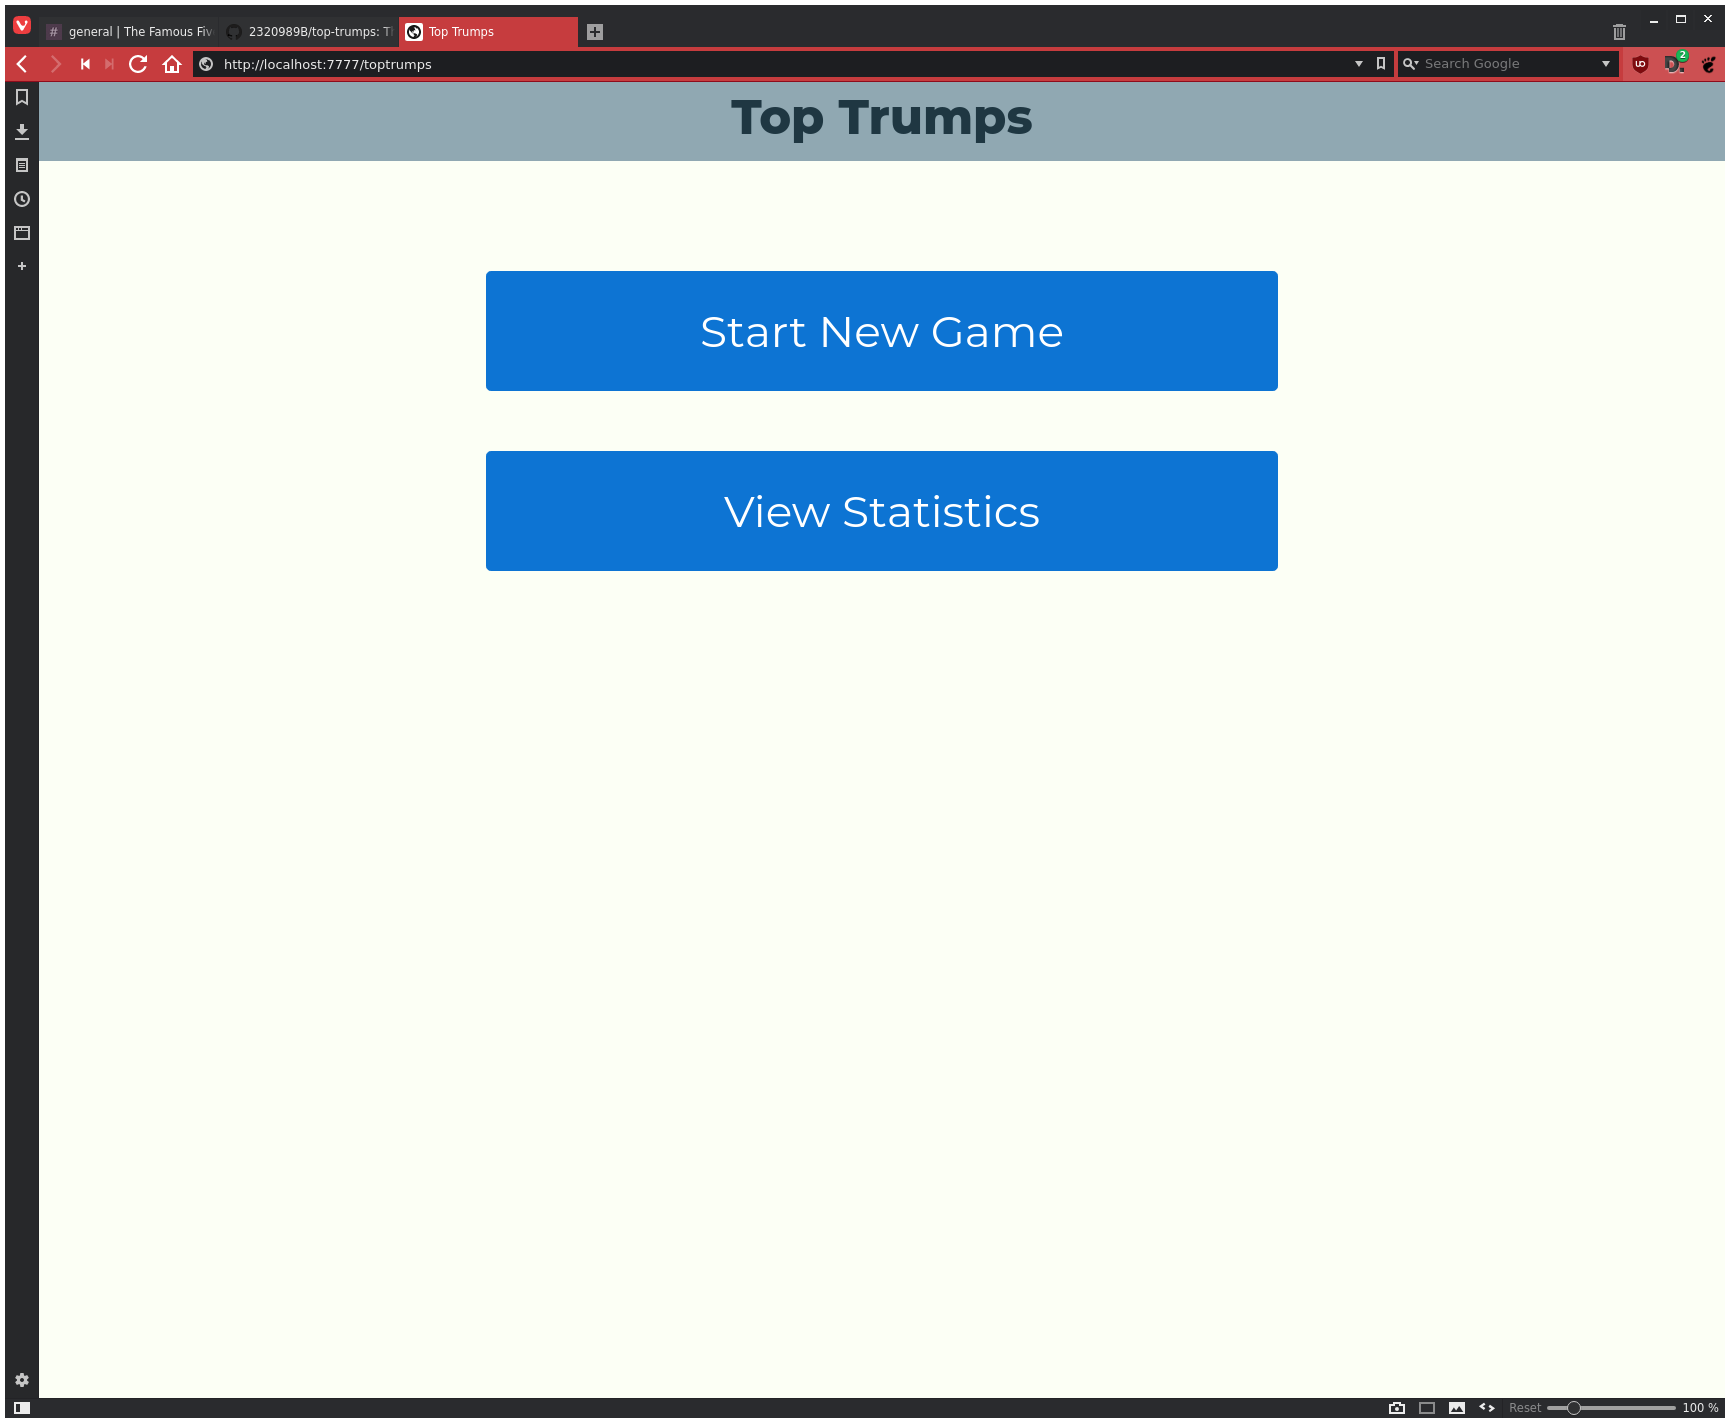
\includegraphics[scale=0.2]{sample.png}
	\captionof{figure}{Main Menu.}
\end{center}

\newpage
\section{Development Process}

	\subsection{Requirements Analysis}

Reference is made to Appendix \ref{appendix:kick_off_mom} for minutes of the project kick-off meeting.
	\subsection{User Stories}

An initial set of user stories were brainstormed by each team member and posted on a Trello board. 
Reference is made to Appendix \ref{appendix:sprint1_planning_meeting} for minutes of the initial planning meeting, where user stories were finalised.
To ensure full coverage of requirements, a \todo{Should we include an updated coverage matrix in an appendix?} coverage matrix was produced to give the team confidence the main aspects were captured.

The final set of user stories can be found in Appendix \ref{appendix:user_stories}.
	\subsection{Design}

An initial design meeting was held to agree overall technical approach.
Reference is made to Appendix \ref{appendix:design_meeting} for further details.
Since this meeting, the design evolved as the team got more familiar with the design challenges.

This section communicates the final design.
Where possible, the team implemented common design patterns in an effort to reduce coupling and to follow best-practices.
Overall architecture makes use of the MVC pattern, applied per Figure \ref{figure:system_architecture}:

\begin{center}
	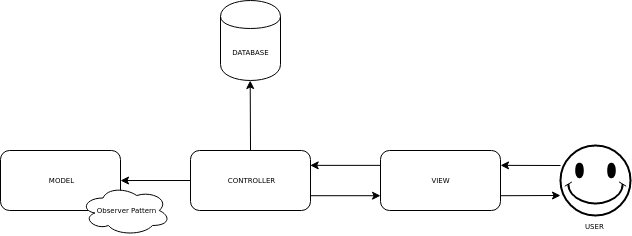
\includegraphics[scale=0.7]{system_architecture}
	\captionof{figure}{System Architecture}
	\label{figure:system_architecture}
\end{center}

The model and database components were designed to be used by either the command line or online modes of the system:

\begin{itemize}
	\item Model (\texttt{package model}, see Figure \ref{figure:model_uml} for UML):
	\begin{itemize}
		\item Encapsulate game actions and game state.
		\item Be agnostic to the implementation of other parts of the system. Apply the Observer Pattern to eliminate any need for the model to be aware of external components, reducing coupling. Passively notify interested parties of changes to game state.
		\item Provide a set of public methods to trigger key game actions (Facade Pattern) (\texttt{GameAPI.java}).
		\item Provide a Immutable Parameter Object to extract a snapshot of key game data from within the model, allowing a single ``info'' object to passed to other parts of the system (\texttt{GameInfo.java}).
	\end{itemize}

	\item Database (\texttt{package persistence}, see Figure \ref{figure:persistence_uml} for UML):
	\begin{itemize}
		\item Provide a set of public methods to write key game information to a persistent database.
	\end{itemize}
\end{itemize}

A specific controller and views were created for command line mode:

\begin{itemize}
	\item Controller (\texttt{package commandline}, see Figure \ref{figure:commandline_uml} for UML):
	\begin{itemize}
		\item Provide game management and logical flow, specific to the command line implementation .
		\item Serve views to user, and trigger necessary game actions.
		\item Trigger game events based on game state (via Observer).
		\item Limit coupling with model by calling \texttt{GameAPI.java} methods only.
	\end{itemize}

	\item View(s) (\texttt{package commandline}, see Figure \ref{figure:commandline_uml} for UML):
	\begin{itemize}
		\item Provide command line output and facilities to retrieve user input, specific to the command line implementation.
		\item Limit coupling by communicating only with the controller.
	\end{itemize}
\end{itemize}

For online mode:

\begin{itemize}
	\item Controller (\texttt{package online}), see Figure \ref{figure:online_uml} for UML):
	\begin{itemize}
		\item Provide game management and logical flow, specific to the online implementation.
		\item Provide APIs for the user to interact with the Game logic via the web page views.
		\item Trigger game events based on user interaction via web pages (i.e. API calls).
		\item Limit coupling with model by calling \texttt{GameAPI.java} methods only.
	\end{itemize}

	\item View(s) (\texttt{package online}), see Figure \ref{figure:online_uml} for UML):
	\begin{itemize}
		\item Provide output and receive user input via (.ftl) web pages specific for the online implementation.
		\item Coupling limited by freeing the web pages from interacting with the Game logic.
	\end{itemize}
\end{itemize}

The interaction between all packages is captured in Figure \ref{figure:full_uml}. 
The native image is also provided with the team .zip submission for readability.

\newpage
\begin{center}
	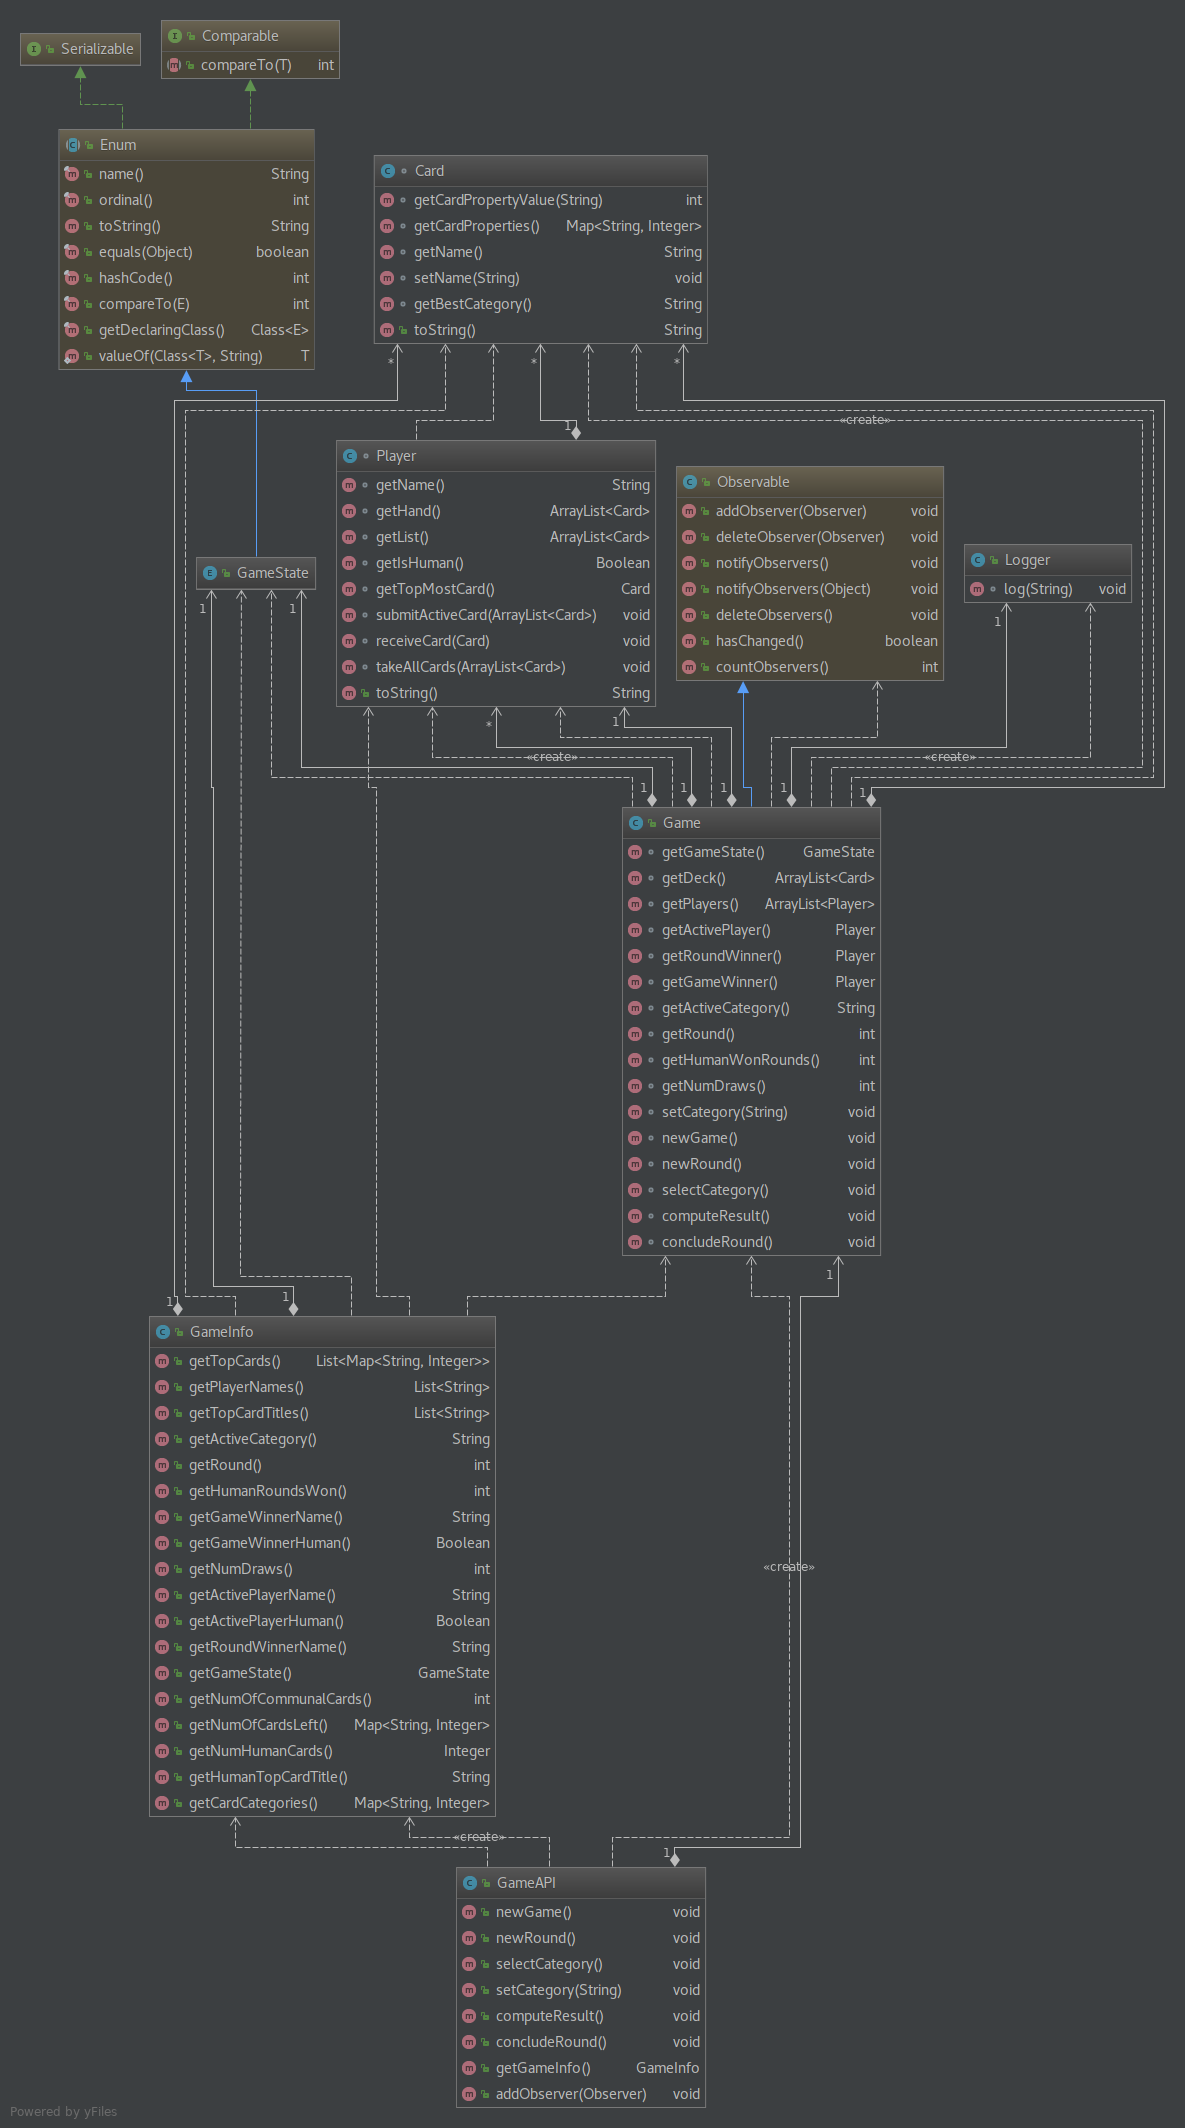
\includegraphics[scale=0.29]{final_UML_model_package}
	\captionof{figure}{Model Package UML (Package Visibility)}
	\label{figure:model_uml}
\end{center}

\begin{center}
	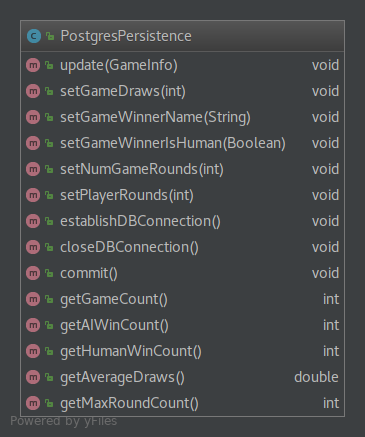
\includegraphics[scale=0.4]{final_UML_persistence_package}
	\captionof{figure}{Persistence Package UML (Package Visibility)}
	\label{figure:persistence_uml}
\end{center}

\begin{center}
	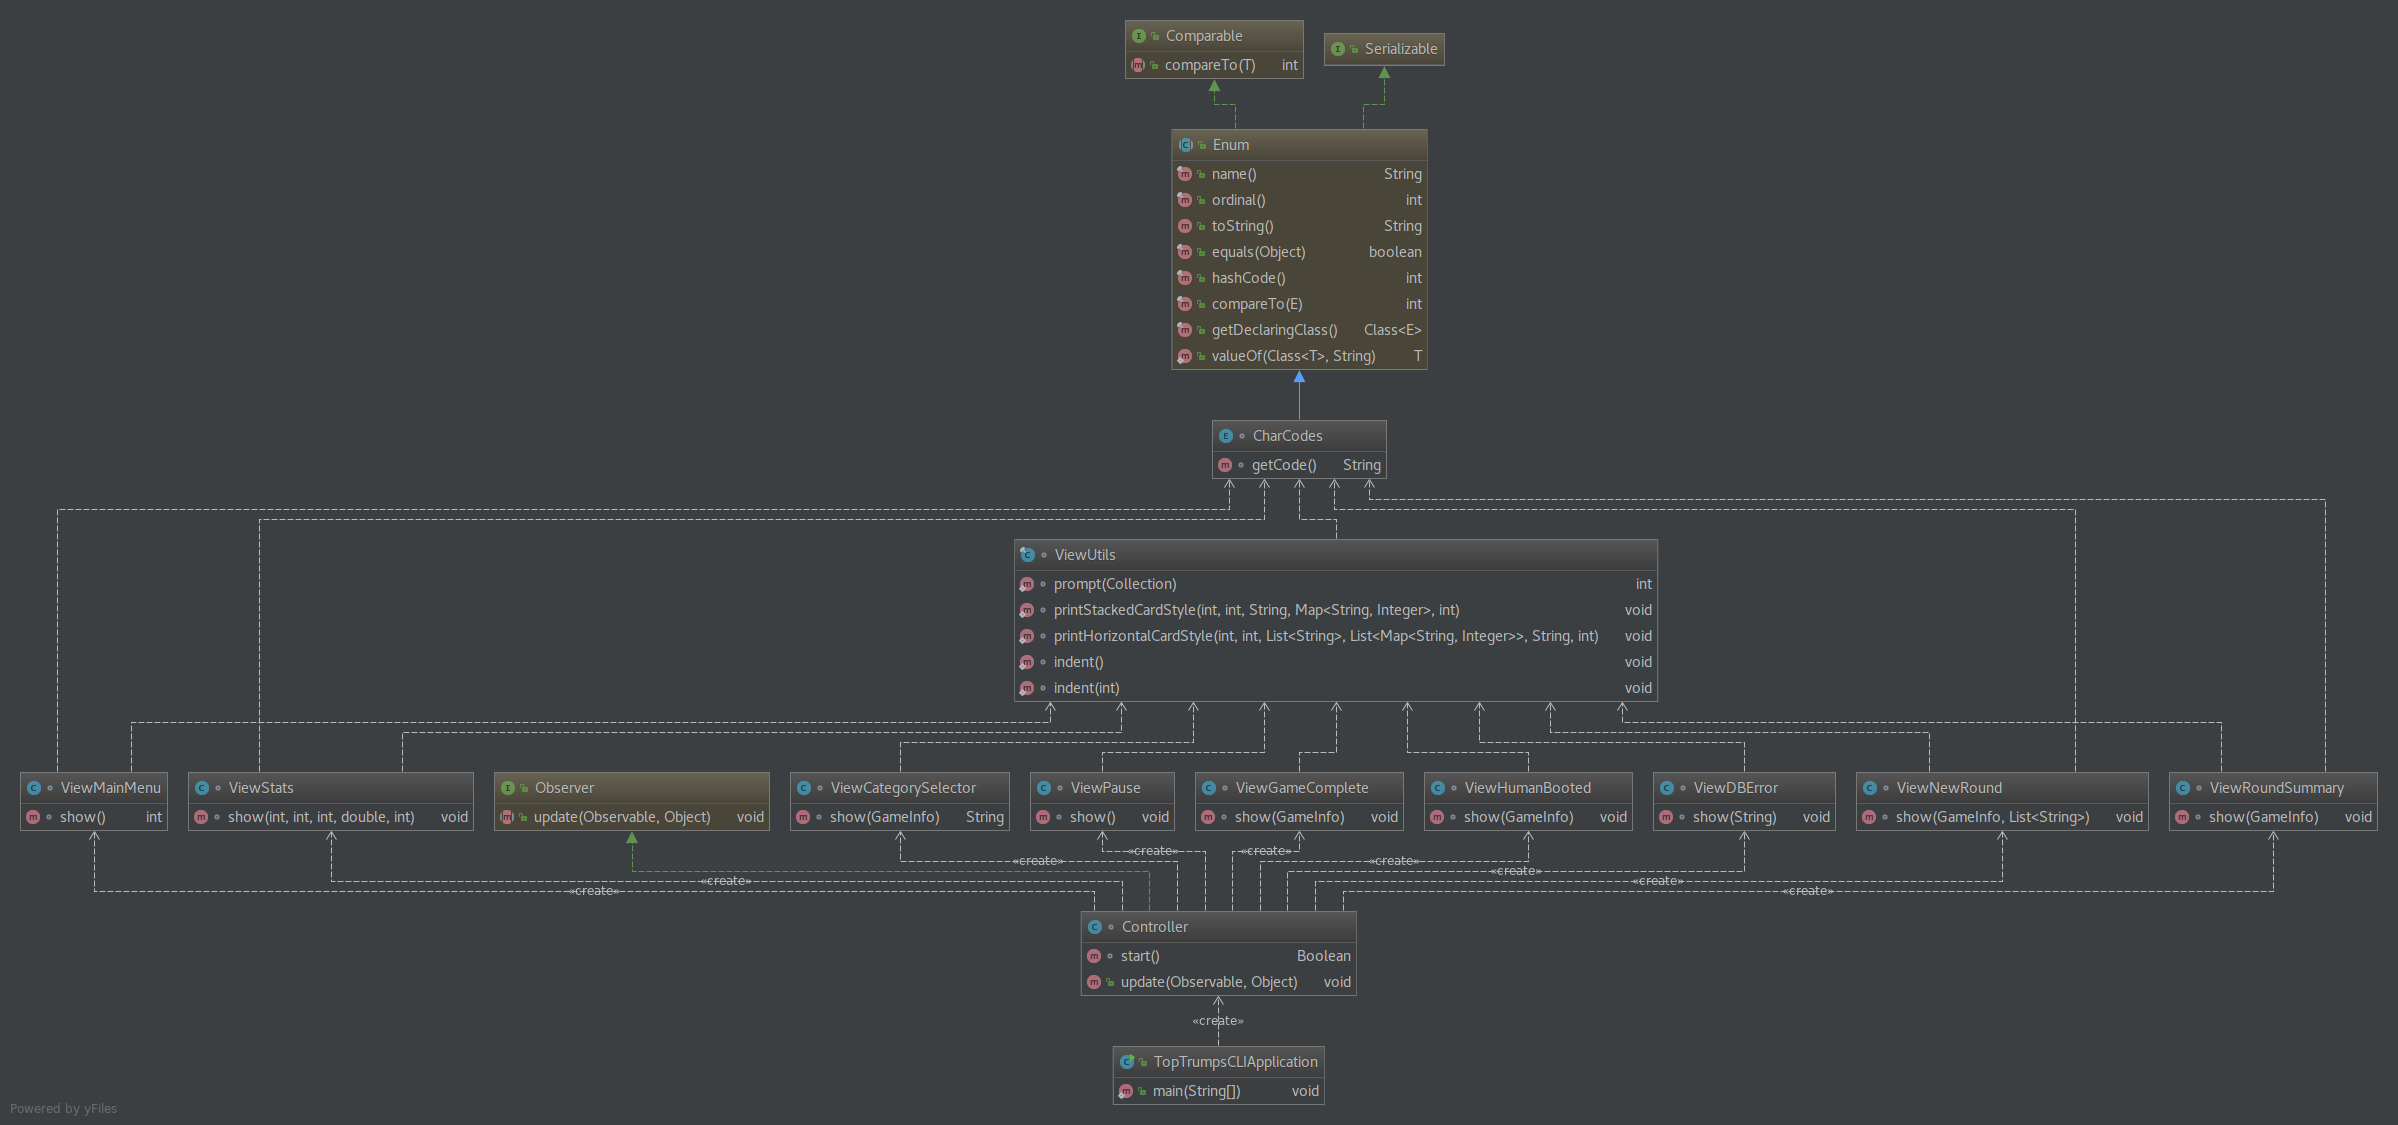
\includegraphics[width=\textwidth]{final_UML_commandline_package}
	\captionof{figure}{Commandline Package UML (Package Visibility)}
	\label{figure:commandline_uml}
\end{center}

\begin{center}
	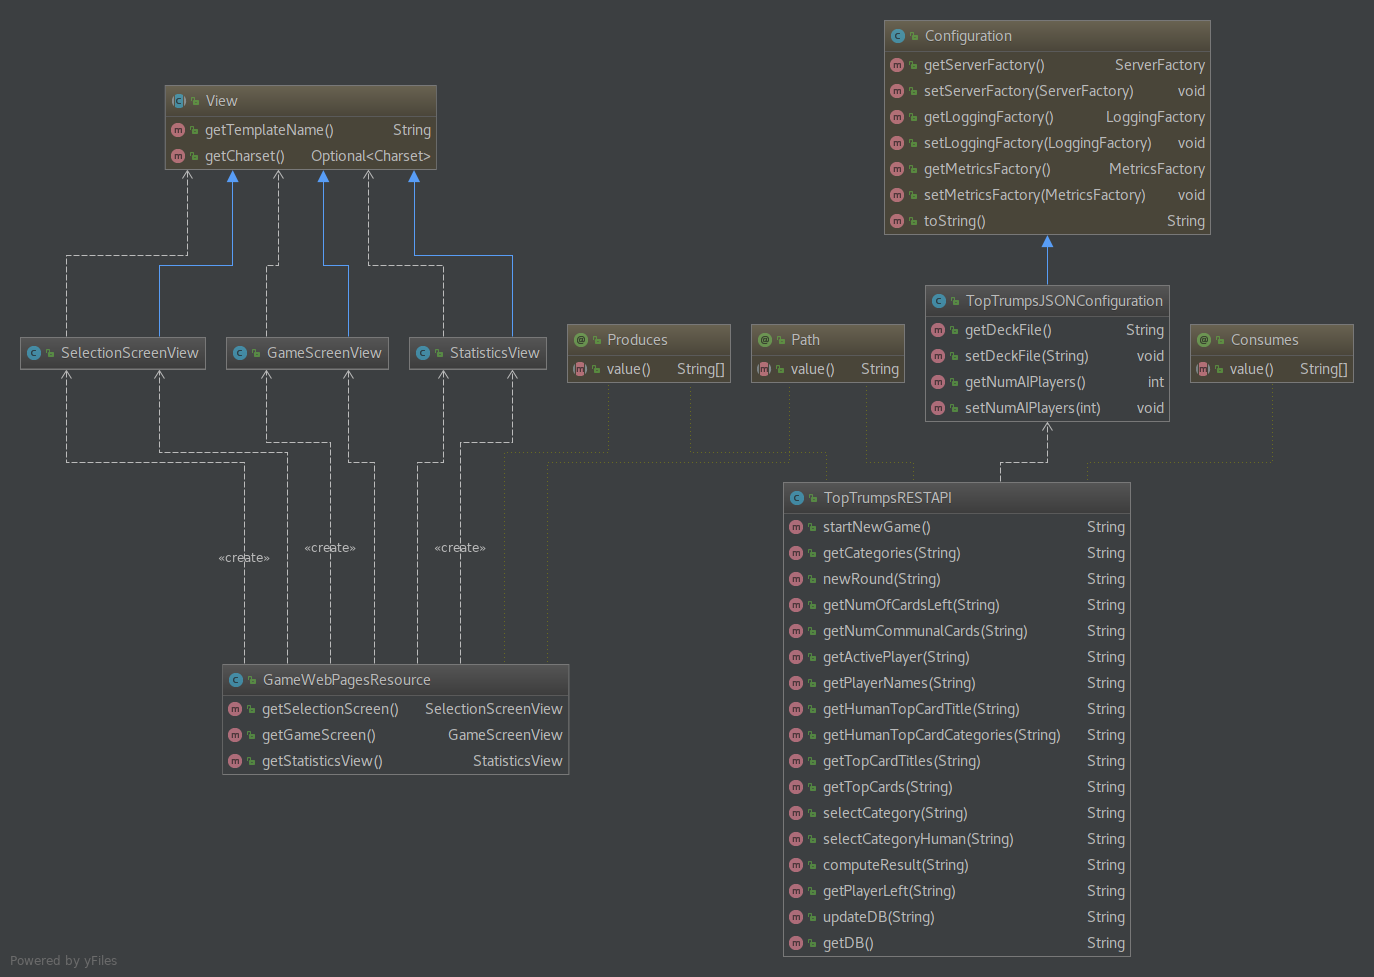
\includegraphics[width=\textwidth]{final_UML_online_package}
	\captionof{figure}{Online Package UML (Package Visibility)}
	\label{figure:online_uml}
\end{center}

\begin{center}
	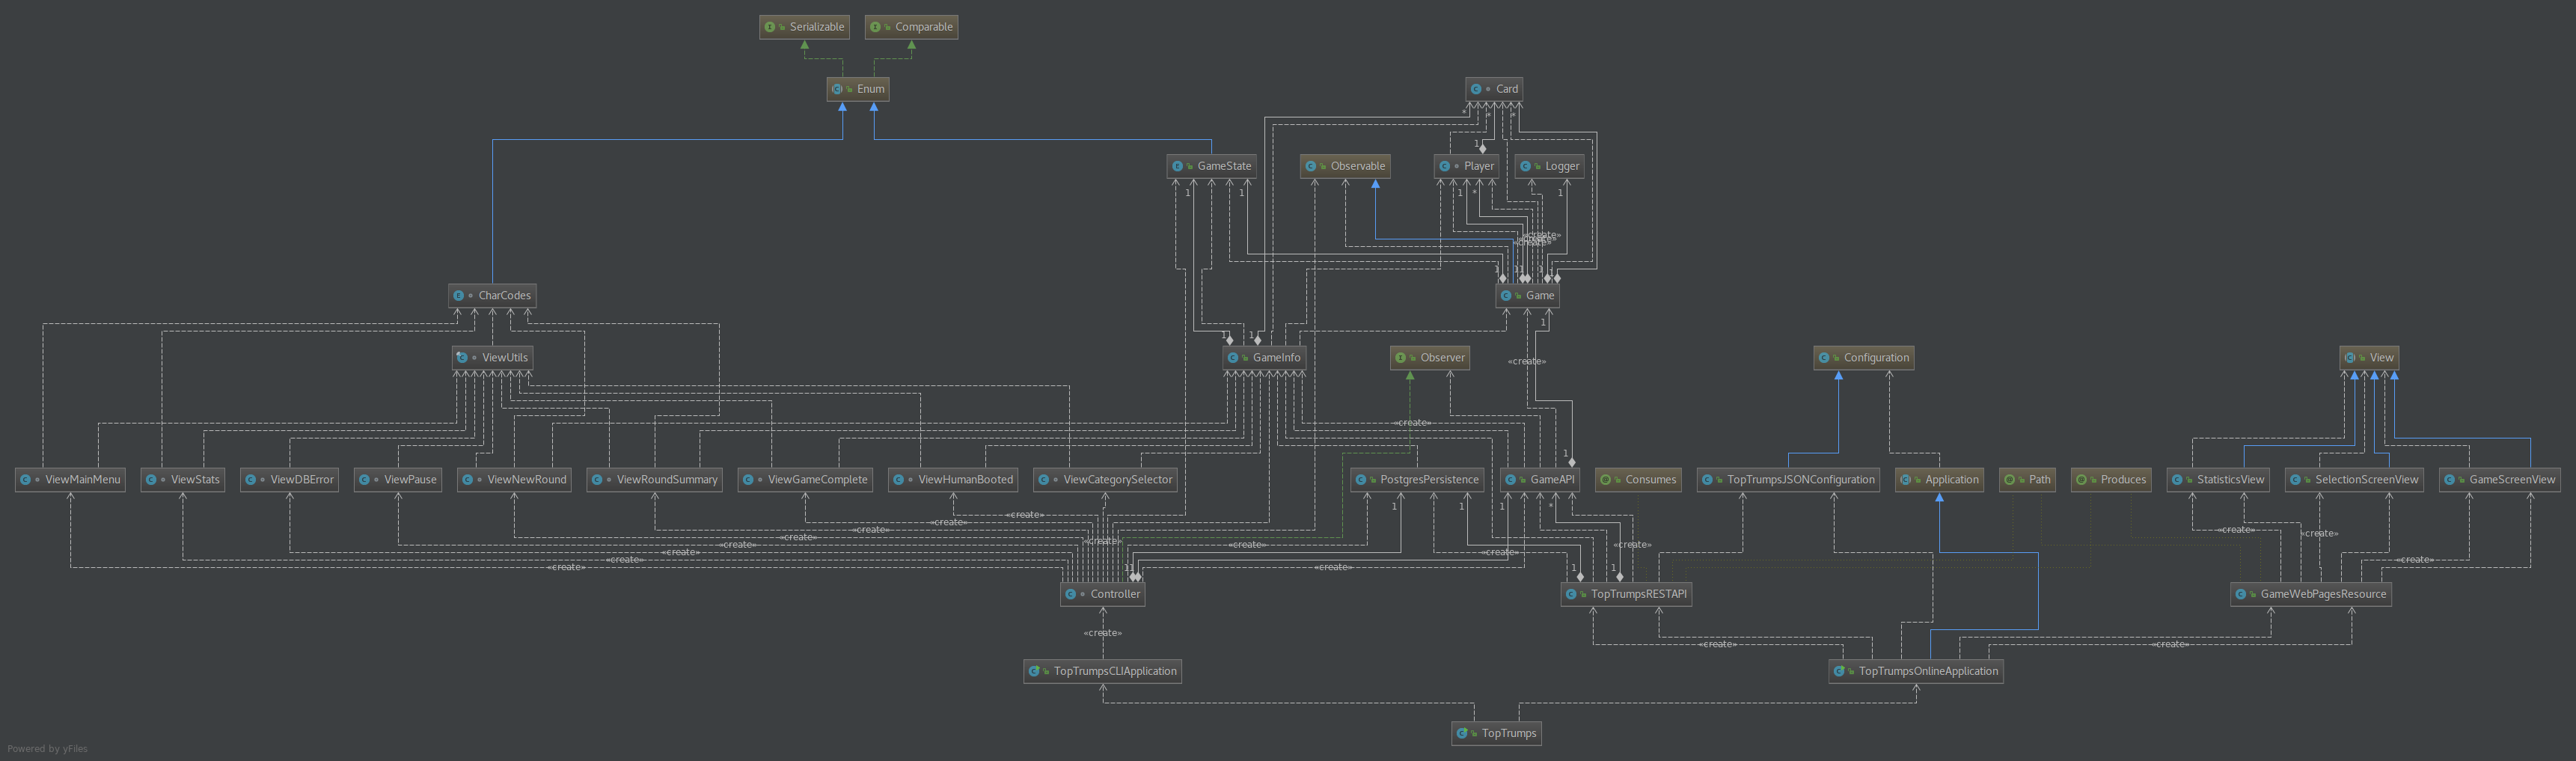
\includegraphics[scale=0.19, angle=90]{final_uml_full}
	\captionof{figure}{Full System UML.}
	\label{figure:full_uml}
\end{center}
	\subsection{Sprints}

\subsubsection{Sprint \#1}

\begin{center}
	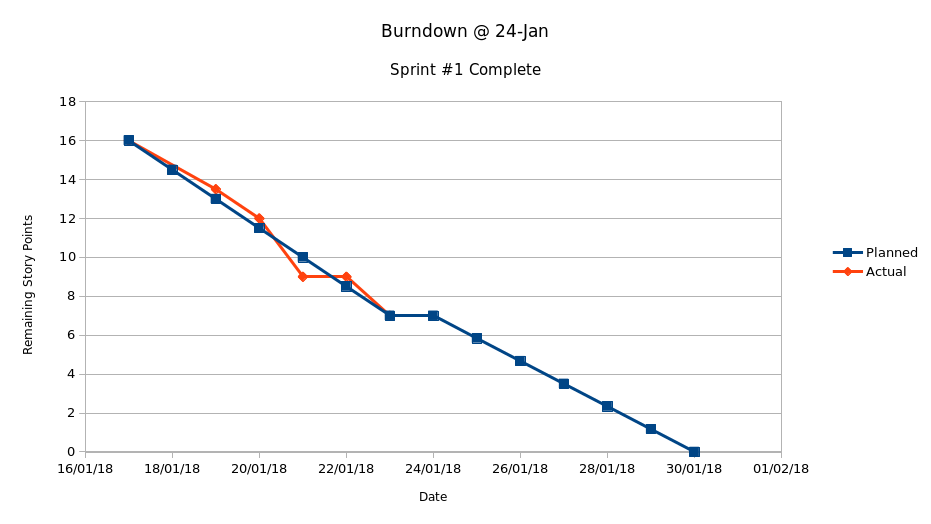
\includegraphics[scale=0.5]{burndown_1}
	\captionof{figure}{Burndown Chart Sprint \#1}
	\label{figure:burndown_1}
\end{center}

The upfront design work paid dividends during Sprint \#1, resulting in steady progress during implementation.
As noted in Appendix \ref{appendix:sprint2_planning_meeting}, some stories took longer than anticipated to complete, however the team stepped-up efforts to complete all stories within the iteration.

\subsubsection{Sprint \#2}

\begin{center}
	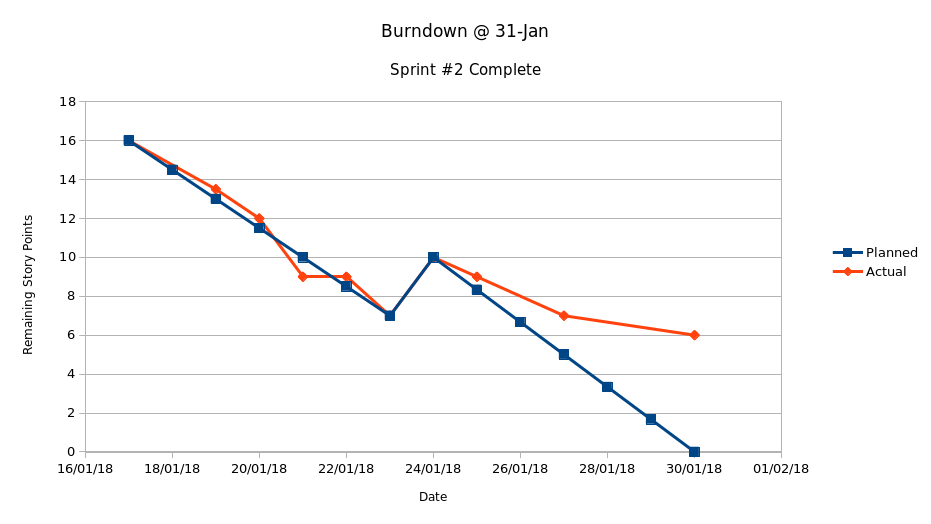
\includegraphics[scale=0.5]{burndown_2}
	\captionof{figure}{Burndown Chart Sprint \#2}
	\label{figure:burndown_2}
\end{center}

Sprint \#2 proved to be a challenge, due to the team's overall lack of experience with the online technologies, and the impact of some early decisions.
During Sprint \#1, the model (specifically the \texttt{Game} class), was implemented in a way that relied on a single flow of events, with most game logic being contained in a single method. When the Observable \texttt{notify()} method was called at key stages to change \texttt{gameState}, execution was blocked, passing execution over to the controller where the event was handled. Upon completion of the controller flow, execution was handed back to the model where the logic continued.

However, due to the asynchronous, stateless nature of the online technologies, this blocking mechanism was no longer available.
The solution was to refactor the model to create individual methods for each segment of game logic, which would be triggered by the controller as needed.
The impact of this was that most stories could not be completed within the iteration, and a third sprint had to be scheduled.

Appendix \ref{appendix:sprint3_planning_meeting} has further details.

\subsubsection{Sprint \#3}

\begin{center}
	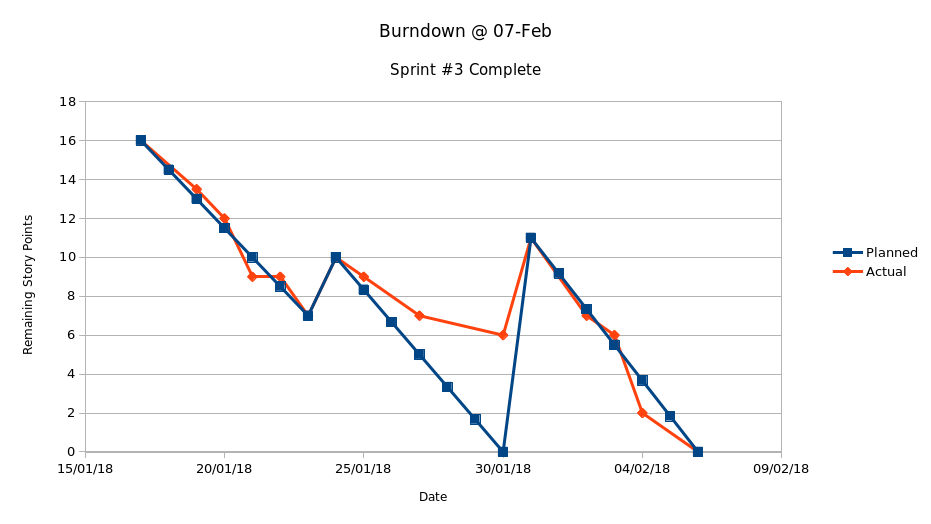
\includegraphics[scale=0.5]{burndown_3}
	\captionof{figure}{Burndown Chart Sprint \#3}
	\label{figure:burndown_3}
\end{center}

Sprint \#3 successfully solved the issues encountered previously, and the project came to a functional conclusion at the end of the iteration.

Appendix \ref{appendix:final_sprint_meeting} has further details.

\newpage
\section{Technical}

	\newpage
\section{Assumptions}

The following section contains an outline of the assumptions that have been made during the development of the product, assumptions that the prospective user should keep in mind.

When players have only one card in their individual decks and the outcome of the current round is a draw, then they lose the game as their cards go to the communal deck of cards. This means that, if the game has only two players left and the above scenario happens, then the winner ends up having less than the total of 40 cards in hand.

Another assumption is that in the case of a draw, the next stage of the game is considered to be a new round and not an extension of the draw round. Last winner player will still choose the category, but the game is between all of the players that are still in the game i.e. the ones that still have cards in their decks, and not only those that had the same category values.

Is should also be noted that an AI player will always select the category that holds the best value on his top most card, and the selection will not be random. That will enhance the realistic feel of the game.

It can also be assumed that after every round the content of the communal deck is being collected by the winner player. This means that for the program, it doesn't matter if the result of a round was a draw or not. If the pile is empty and there is a winner, all players submit their cards in the empty pile and the winner player gets the cards from the round back. If the pile is non empty (i.e. the previous round resulted to a draw), then the winner still gets the current cards and the ones that were previously submitted because of the draw.

Another point that should not surprise a potential gamer, is that, if a player has only one card in hand and wins the current round, then his winning card will still be on top for the next round to come. That happens because the winner collects the cards from the other players and puts them at the back of his deck. Since he, had only one card to play with, this card remains on top by default. Again, that will only happen in the case of one card in hand and a winning result for this card holder. 

The online mode assumes that once the player has pressed the button for selecting a category, he cannot change his mind and chose another one. That is, his option has been saved and the only available next step is to show the outcome of the round.

In command line, after the player has selected the category he wants to play with, his choice is only saved after pressing ``enter'', so he has the chance to change the category before selecting to proceed to the next step.



	\newpage
\section{Functionality}
The functionality laid out by the program specification was largely the same across both modes -- command line and online -- with some additional individual functionality required by each.

\subsection{Game Logic}
The logic of the Top Trumps game was implemented as specified. A shuffled deck of cards is distributed in turn to each player until all have been given out. One player will be human controlled with up to 4 AI players. Each card has 5 categories each with a positive integer value. The first active player is selected and chooses a category. All the card values are then revealed along with the winner (the holder of the card with the highest value). The winner takes all the cards in play and is the active player for the next turn. In the event of a draw, all the cards are added to a communal pile which will be won by the winner of the next round in addition to the cards in play.

\subsection{Persistent Game Data}
Both modes were required to communicate with a database in order to store persistent data about gameplay. The user is provided with the total number of games played, the number of human and AI wins, the average number of draws per game and the longest game played (in number of rounds). This was achieved using PostgreSQL. The database schema (appendix X - schema file) allowed the required information to be saved and provided to the user. 

\subsection{Command Line Mode}
The command line opens with a menu asking if the user wants to see past statistics from the database or play a new game. Each round of a new game the user is provided with the round number, the active player and the human player's top card. The game logic is then followed and the user is informed who the round winner is before the next round commences. The number of communal cards is given in the event of a draw. If the user is eliminated the game runs to completion automatically. Once the game is completed the user is sent back to the menu and the database is updated with the game statistics. \\

The command line displays the game information in plaintext and allows the user to enter simple text commands via a numbered interface. \\

\newpage

The command line also offers a test log function, whereby the following is logged:
\begin{itemize}
\item The contents of the deck when read
\item The contents of the deck when shuffled
\item The contents of all player decks when dealt
\item The contents of the communal pile when altered
\item The contents of the players card in play for each round
\item The category selected
\item The contents of each player's deck at round end
\item The winner of the game
\end{itemize}

This output is saved to a text file. \\

The command line functionality requirements were met fully as shown below:
\missingfigure{Command line stats screenshot required.}
\missingfigure{Command line game screenshot required.}
\missingfigure{Command line winner screenshot required.}

\subsection{Online Mode}
The online mode hooks into the same game logic as the command line mode through API calls, however calls for different and more complex user interface functionality. The requirements for this interface were:
\begin{itemize}
\item A 'menu' page, similar to the command line, where the user selects either 'New Game' or 'View Statistics'
\item The user is shown their own top card and allowed to select the category via buttons when it is their turn
\item The user is shown who's turn it currently is
\item The interface should clearly show every player's cards after a category is selected and highlight the winner
\item The user should be informed when the round resulted in a draw
\item The user shold be able to see how many cards are left in each player's deck and the communal deck
\item The winner should be indicated at the end of the game
\end{itemize}

These requirements were fully satisfied by the implementation as shown below:
\missingfigure{Online menu screenshot.}
\missingfigure{Online gameplay screenshot.}
\missingfigure{Online DB screenshot.}


	\newpage
\section{Testing}
\subsection{Command Line Mode}
The tests have been derived from the user stories. It is necessary to mention that the presented tests are from the user point of view, while there were numerous tests at the back-end during the development of the program that are not included. \\
\vspace{0.1cm}\\
The user persona Bob, wants to play a Top Trumps game in the command line.    
\vspace{0.2cm}\\
\begin{tabular}{l | p{12cm}}
User Story & \textbf{S0010} \\
\hline
Type of Test & Initiate the game from command line\\
\hline
Used Variable & 
 - "java -jar ITSD2018Project-1.0.jar -c" \\
 & 
 - "java -jar ITSD2018Project-1.0.jar -c -t"
\\
\hline
Result & [Passed] The program returns the main menu to the player, (figure 1 Appendix). As shown above, both game options were used as variables to test the initialisation of the game.\\ 
\hline
Anti-Variables & - "java -jar ITSD2018Project-1.0.jar -command"\\
& - "java -jar ITSD2018Project-1.0.jar -c -o"\\
& - "java -jar ITSD2018Project-1.0.jar -n"...\\
\hline
Results & [Exception] The program never initiates the game, if the flag is anything else excepts "-c", "-c -t" or "-o". The program throws an exception in case where the user tries to operate both modes, command line mode and on-line mode. In all other cases the program shows the greeting message and terminates.\\
\hline
Reference & Figure \ref{figure:gameInit_true} and \ref{figure:gameInit_false}\\ \hline 
\end{tabular}\\
\vspace{0.2cm}\\ 
The user persona Bob can now select one of the three options of the game.\\
\vspace{0.2cm}\\
\begin{tabular}{l | p{12cm}}
User Story & \textbf{S0010}\\ \hline
Type of Test & Select an integer number from the provided options of the main menu.\\ \hline
Used Variables & - integer number, where n=[1,3].\\ \hline
Result & [Passed] The player enter the integer n=1, which initiates a new game. The program returned with a new game.\\ \hline
Anti-Variables & - String\\
& - Character\\
& - Double or Integer, where n!=[1,3]\\
\hline
Results & [Exception] The program throws an exception when the player does not enter the specified integer between n = [1,2,3]. In case the player enters a different integer, the program throws a message indicating the exact integer variable, where in all other situations the program prints out a message demanding an integer.\\ \hline 
Reference & Figure \ref{figure:mainMenu_true} and \ref{figure:mainMenu_false}\\ \hline
\end{tabular}\\
\vspace{0.2cm}\\
After the proper response of Bob to the game commands, he excepts from the game to load the cards, shuffle them, and divide to all players as equally as possible.\\
\vspace{0.2cm}\\
\begin{tabular}{l | p{12cm}}
User Story & \textbf{S0020}\\ \hline
Type of Test & Examination of the test log file for the correct loading of deck, correct shuffling and dividing.\\ \hline
Used Variables & No variables for this test.\\ \hline
Result & [Passed] The program does the deck loading, shuffling, creating players' deck and choose randomly the active player correctly. \\ \hline
Anti-Variables & \textit{No anti-variables for this test} \\ \hline
Results & \textit{[No Exception] There is no results for this test.} \\ \hline
Reference & Figure \ref{figure:gameInit_true} and \ref{figure:testlog}\\ \hline
\end{tabular}\\
\vspace{0.2cm}\\
Bob wants to have a detailed round and understand who is active player, which category is selected and who won the round.\\
\vspace{0.2cm}\\
\begin{tabular}{l | p{12cm}}
User Story & \textbf{S0030} \& \textbf{S0040} \\ \hline
Type of Test & Game round quality test.\\ \hline
Used Variables & - Press Enter button to show winner\\ \hline
Result & [Passed] The program shows the round number, who is active player, all the cards that participate in this specific round, the selected category inside square brackets and the round winner.\\ \hline
Anti-Variables & \textit{No anti-variables for this quality test} \\ \hline
Results & [\textit{No Exception]} there is no exception for this test, only through the test log file. \\ \hline
reference & Figure \ref{figure:cmd_winner}, \ref{figure:cmd_play} and \ref{figure:falseInput}
\\ \hline
\end{tabular}\\
\vspace{0.2cm}\\
Bob, who is an expert user of command line, wants to have a record of the entire game in details in a test log file. He is able to do so, with the -t flag when he initiate the game\\
\vspace{0.2cm}\\
\begin{tabular}{l | p{12cm}}
User Story & \textbf{S0050}\\ \hline
Type of Test & Run the game with the "-t" flag.\\ \hline
Used Variables & - "java -jar ITSD2018Project-1.0.jar -c -t"\\ \hline
Result & [Passed] The program recognise the -t flag and checks if there is no file as "toptrumps.txt" log file, it creates one, or it rewrites in the existing one.\\ \hline
Anti-Variables & - "java -jar ITSD2018Project-1.0.jar -c -*", where * is anything else than "-t".\\ \hline
Results & \textit{[No Exception]} The program recognise the -c flag but it does not produce or write in the "toptrumps.txt" file. \\ \hline
Reference & Figure \ref{figure:gameInit_true} and \ref{figure:testlog}\\ \hline
\end{tabular}\\
\vspace{0.2cm}\\
Bob is very cautious about the validity of the game. As a result he wants to examine who won the round and if the AI player selected the highest attribute.\\
\vspace{0.2cm}\\
\begin{tabular}{l | p{12cm}}
User Story & \textbf{S0130} \\ \hline
Type of Test & Print players top cards. Quality test \\ \hline
Used Variables & \textit{No variables used to this test}\\ \hline
Result & [Passed] The program prints out the top cards from all available players. Moreover, the program shows the selected category.\\ \hline
Anti-Variables & \textit{No anti-variables used for this test.}\\ \hline
Results & \textit{[No Exception] There is no exception for this test.}\\ \hline
Reference & Figure \ref{figure:cmd_winner} \\ \hline
\end{tabular}\\
\vspace{0.2cm}\\
Bob is the active player in the game and wants to select a category. The program provides him with the option to enter a integer number that matches a specific category.\\
\vspace{0.2cm}\\
\begin{tabular}{l | p{12cm}}
User Story & \textbf{S0030}\\ \hline
Type of Test & Human Player is active player and selects a category\\ \hline
Used Variables & Integer number n=[1,5]\\ \hline
Result & [Passed] The program receives the input integer variable and makes the desired category active. Then, it returns to the system out the results of the round.\\ \hline
Anti-Variables & String, Characters, Double or Integer variables except n=[1,5].\\ \hline
Results & [Exception] The program throws an exception when the human player did not enter one of the five options. The program catches NULL values, strings, characters, doubles and integer number except the n=[1,5]\\ \hline
Reference & Figure \ref{figure:cmd_play} and \ref{figure:falseInput} \\ \hline
\end{tabular}\\
\vspace{0.2cm}\\
Bob continues his game and he managed to eliminate some of the players, but he wants to know who has been eliminated.\\
\vspace{0.2cm}\\  
\begin{tabular}{l | p{12cm}}
User Story & \textbf{S0040}\\ \hline
Type of Test & Show who players have been eliminated while the human player is in the game. Quality test.\\ \hline
Used Variables & \textit{No variables used for this test.}\\ \hline
Result & [Passed] The program prints out a list with all the active players of the game in each round, right above the players hand.\\ \hline
Anti-Variables & \textit{No anti-variables used for this test.}\\ \hline
Results & \textit{[No exception] There is no exception for this test.}\\ \hline
Reference & Figure \ref{figure:eliminated} \\ \hline
\end{tabular}\\
\vspace{0.2cm}\\
Bob has finished his game and wants to see the game statistics.\\
\vspace{0.2cm}\\  
\begin{tabular}{l | p{12cm}}
User Story & \textbf{S0180}\\ \hline
Type of Test & Show the game statistics.\\ \hline
Used Variables & \textit{No variables used for this test.}\\ \hline
Result & [Passed] The program prints out a list with all the active players of the game in each round, right above the players hand.\\ \hline
Anti-Variables & \textit{No anti-variables used for this test.}\\ \hline
Results & \textit{[No exception] There is no exception for this test.}\\ \hline
Reference & Figure \ref{figure:cmd_stats} \\ \hline
\end{tabular}\\
\subsection{Online Mode}
\vspace{0.2cm} 
The user persona Lilly wants to play a game of Top Trumps online.\\
\vspace{0.2cm}\\  
\begin{tabular}{l | p{12cm}}
User Story & \textbf{S0200}\\ \hline
Type of Test & Initiate the game from command line to play online.\\ \hline
Used Variables & String - "java -jar ITSD2018Project-1.0.jar -o" \& "http://localhost:7777/toptrumps"\\ \hline
Result & [Passed] The first indication of the successful connection to the local server is from the command window. The second indication is by entering the url to the browser.\\ \hline
Anti-Variables & String - "java -jar ITSD2018Project-1.0.jar -*"\\ \hline
Results & [Exception] There is no message of connection with the server in the command window. Also, the browser cannot find the url.\\ \hline
Reference & Figure \ref{figure:onlineMode} and \ref{figure:online_menu} \\ \hline
\end{tabular}\\
\vspace{0.2cm}\\
Lilly wants to press the statistics button and check the game stats, instead of start a new game.\\
\vspace{0.2cm}\\  
\begin{tabular}{l | p{12cm}}
User Story & \textbf{S0190} \& \textbf{S0210}\\ \hline
Type of Test & Quality test. Check the "View Stats" button from the main menu for online mode.\\ \hline
Used Variables & "View Stats" button press.\\ \hline
Result & [Passed] The program opens the statistics view correctly and shows the game stats after a successful CORS call.\\ \hline
Anti-Variables & \textit{No anti-variables used for this test}\\ \hline
Results & \textit{[No Exception] there is no exception for this test.}\\ \hline
Reference & Figure \ref{figure:online_stats}\\ \hline
\end{tabular}\\
\vspace{0.2cm}\\
Lilly has decided to play a new game. The program changes the selection view with the game screen view.\\
\vspace{0.2cm}\\  
\begin{tabular}{l | p{12cm}}
User Story & \textbf{S0220}\\ \hline
Type of Test & Quality test. Check the "New Game" button from the main menu for online mode.\\ \hline
Used Variables & "New Game" button press.\\ \hline
Result & [Passed] The program successfully opens the game screen view with a new game initialised. The program shows the player's card, who is active player, the current round and the number of cards in the communal pile.\\ \hline
Anti-Variables & \textit{No anti-variables used for this test.}\\ \hline
Results & \textit{[No exception] there is no exception for this test.}\\ \hline
Reference & Figure \ref{figure:readyStart} \\ \hline
\end{tabular}\\
\vspace{0.2cm}\\  
Lilly is ready to play and he wants to know what category is selected by the other players.\\
\vspace{0.2cm}\\
\begin{tabular}{l | p{12cm}}
User Story & \textbf{S0220}\\ \hline
Type of Test & Quality test. Check if the game proceeds if the human in not the active player.\\ \hline
Used Variables & "Category Selection" button press.\\ \hline
Result & [Passed] The program process the data and returns the the cards of all players that are still in the game, which category had been selected and who won the round.\\ \hline
Anti-Variables & Check "Categories" are locked.\\ \hline
Results & [Exception] While the human player is not the active player, she cannot select a category.\\ \hline
Reference & Figure \ref{figure:online_play} \\ \hline
\end{tabular}\\
\vspace{0.2cm}\\  
Lilly has won a round and wants to select a category from her card.\\
\vspace{0.2cm}\\ 
\begin{tabular}{l | p{12cm}}
User Story & \textbf{S0220 \& S0230}\\ \hline
Type of Test & Press one category button and then the "Select Category" button to proceed.\\ \hline
Used Variables & "Select Category" button press\\ \hline
Result & [Passed] The program store the selected category and waits until the player press the "Select Category" button. After that the round proceed as is, with the calculation of the winner.\\ \hline
Anti-Variables & \emph{No anti-variables used for this test.}\\ \hline
Results & \emph{[No exception] There is no exception for this test.}\\ \hline
Reference & Figure \ref{figure:online_selectCategory} and \ref{figure:online_humanRound} \\ \hline
\end{tabular}\\
\vspace{0.2cm}\\
After several rounds, Lilly has encounter a draw. However, she wants to know how many cards are in the communal pile and that the outcome of the round was a draw.\\
\vspace{0.2cm}\\   
\begin{tabular}{l | p{12cm}}
User Story & \textbf{S0240}\\ \hline
Type of Test & Check if the program prints the draw and updates the communal pile.\\ \hline
Used Variables & "Show Winner" press button.\\ \hline
Result & [Passed] the program prints successfully the draw and updates the communal pile with the player cards.\\ \hline
Anti-Variables & \emph{No anti-variables used for this test.}\\ \hline
Results & \emph{[No exception] There is no exception used for this test.}\\ \hline
Reference & Figure \ref{figure:drawOnline} \\ \hline
\end{tabular}\\
\vspace{0.2cm}\\
Lilly has eliminated from the game and wants to complete this game.\\
\vspace{0.2cm}\\  
\begin{tabular}{l | p{12cm}}
User Story & \textbf{S0250}\\ \hline
Type of Test & Use an auto-complete button to complete the game, when the human is eliminated.\\ \hline
Used Variables & "Auto Complete" button press.\\ \hline
Result & [Passed] The program simulates the rest of the game without the human interaction until the winner is decided.\\ \hline
Anti-Variables & \emph{No anti-variables used for this game.}\\ \hline
Results & \emph{[No exception] There is no exception used for this test}\\ \hline
Reference & Figure \ref{figure:autoComplete} \\ \hline
\end{tabular}\\
\vspace{0.2cm}\\
Lilly has won her game and wants to return to the main menu.\\
\vspace{0.2cm}\\  
\begin{tabular}{l | p{12cm}}
User Story & \textbf{S0250}\\ \hline
Type of Test & Check that the program return the screen view to the Main Menu.\\ \hline
Used Variables & There is no button for this test.\\ \hline
Result & [Passed] The program identifies the end of the game and redirect the screen view to the Selection screen.\\ \hline
Anti-Variables & \emph{No anti-variables used for this test.}\\ \hline
Results & \emph{[No exception] There is no exception for this test.}\\ \hline
Reference & Figure \ref{figure:online_menu} \\ \hline
\end{tabular}\\
\vspace{0.2cm}\\
Lilly is really up to the game and wants to play simultaneously different games.\\
\vspace{0.2cm}\\  
\begin{tabular}{l | p{12cm}}
User Story & \textbf{S0200}\\ \hline
Type of Test & Check that the program can handle multiple games simultaneously.\\ \hline
Used Variables & "http://localhost:7777/toptrumps/" in different tabs.\\ \hline
Result & [Passed] The program can have multiple games at the same time.\\ \hline
Anti-Variables & \emph{No anti-variables used for this test.}\\ \hline
Results & \emph{[No exception] There is no exception for this test.}\\ \hline
Reference & Figure \ref{figure:multipleGames} \\ \hline
\end{tabular}\\

	\newpage
\subsection{Deficiencies}

The program has been tested thoroughly, during different steps of development, after every sprint in a larger scale, and as a final complete product multiple times. No missing functionality has been observed, and all tests were passed. 

Minor points can be mentioned, but again they are not part of functionality and they do not affect the program in any way. For example, in command line mode, cards are represented graphically as rectangles. If the user tries to reduce the terminal window size below a certain point, the rectangles overlap and do not re-shape automatically to fit the window. It is assumed though, that player would not want to run the game in a very small terminal,so that should not be an issue. Perhaps this would be something to adjust if the period available for the project completion was a little longer.


\begin{appendices}
	\newpage
\section{Minutes of Meeting}


\subsection{Project Kick-Off}
\label{appendix:kick_off_mom}

\momtoptable
{Fri 12-Jan 2018 (Week 1)}
{Boyd Orr}
{Christopher Bellingham}
{Ioannis Athanasiadis [IA]\newline
Christopher Bellingham [CB]\newline
Joseph Doogan [JD]\newline
Pavlos Evangelidis [PE]\newline
Torquil MacLeod [TM]}
{-}

\begin{momitems}
	% Item, Details, Resp., Due.
	\momitem
	{1}
	{Team reviewed and approved Team Organisation Document.}
	{INFO}
	{INFO}

	\momitem
	{2}
	{Publish latest Team Organisation Document to Slack to allow each team member to submit to Moodle.}
	{CB}
	{Fri 12-Jan}

	\momitem
	{3}
	{Create Customer Specification, capturing all requirements. Post-meeting note, see Appendix \ref{appendix:customer_specification}.}
	{CB}
	{Sun 14-Jan}

	\momitem
	{4}
	{Populate Trello with User Stories based on Customer Spec prior to Sprint Planning meeting on Wed-17.}
	{ALL}
	{Wed 17-Jan}

	\momitem
	{5}
	{Consider architecture and high-level Object Orientated design prior to Design meeting on Wed-17.}
	{ALL}
	{Wed 17-Jan}
\end{momitems}


\newpage
\subsection{Sprint Planning Meeting}
\label{appendix:sprint1_planning_meeting}

\momtoptable
{Wed 17-Jan 2018 (Week 2)}
{Slack}
{Christopher Bellingham}
{Ioannis Athanasiadis [IA]\newline
Christopher Bellingham [CB]\newline
Joseph Doogan [JD]\newline
Pavlos Evangelidis [PE]\newline
Torquil MacLeod [TM]}
{-}

\begin{momitems}
	% Item, Details, Resp., Due.
	\momitem
	{1}
	{User stories submitted to Trello were reviewed. Duplicate stories were eliminated, remaining stories were allocated durations.}
	{INFO}
	{INFO}
	
	\momitem
	{2}
	{Unique Story IDs were granted to each User Story, in the form SXXXX. This will aid communication as development progresses.}
	{INFO}
	{INFO}

	\momitem
	{3}
	{Team agreed to define each story as a Must Have, since all generated stories are strictly limited to the requirements of the specification. The team reserves the right to de-prioritise individual stories should the workload be considered too high.}
	{INFO}
	{INFO}

	\momitem
	{4}
	{The sum of all story points is 16. Broadly, Team feels development can be split into two main phases - command line mode, and online mode. Resultant stories can be found in Appendix \ref{appendix:user_stories_command_line} and Appendix \ref{appendix:user_stories_online} respectively.}
	{INFO}
	{INFO}

	\momitem
	{5}
	{Command line mode covers stories S0010, S0020, S0030, S0040, S0050, S0130, S0180. This equates to a total of 9 story points.}
	{INFO}
	{INFO}

	\momitem
	{6}
	{Online mode covers stories S0190, S0200, S0210, S0220, S0230, S0240, S0250. This equates to a total of 7 story points.}
	{INFO}
	{INFO}

	\momitem
	{7}
	{Development of command line and online mode will be tackled over the course of two 1-week long sprints. With consideration for the need for sprint planning/retrospectives, this leaves 6 days per sprint. Each team member's capacity was assumed to be one third of this duration, I.e. 2 ideal days each. Considering a team size of 5, total available capacity per sprint is 10 ideal days.}
	{INFO}
	{INFO}

	\momitem
	{8}
	{With consideration of team capacity, it is deemed feasible to tackle the project over the course of two 1-week sprints. Sprint 1 will tackle command line mode. Sprint 2 will tackle online mode.}
	{INFO}
	{INFO}

	\momitem
	{9}
	{With initial consideration to an MVC-style architecture, it was noted that each story may slice through multiple layers of this architecture. Team considers it sensible for individuals to have responsibility over different segments of the system, as such each user story will be split between multiple developers. Allocation of user stories to individuals will therefore be deferred until this afternoon's design meeting, where architecture and class structure will be finalised.}
	{INFO}
	{INFO}

	\momitem
	{10}
	{Project schedule was created, allowing for 6-days float/contingency prior to report submission (Figure \ref{figure:initial_project_plan}).}
	{INFO}
	{INFO}

	\momitem
	{11}
	{It was agreed that the requirements presented in Appendix \ref{appendix:customer_specification} should be cross-referenced to each user story, to ensure full coverage of requirements. A coverage matrix will be produced by the team to confirm there are no coverage gaps.}
	{ALL}
	{Fri 19-Jan}
\end{momitems}

\begin{center}
	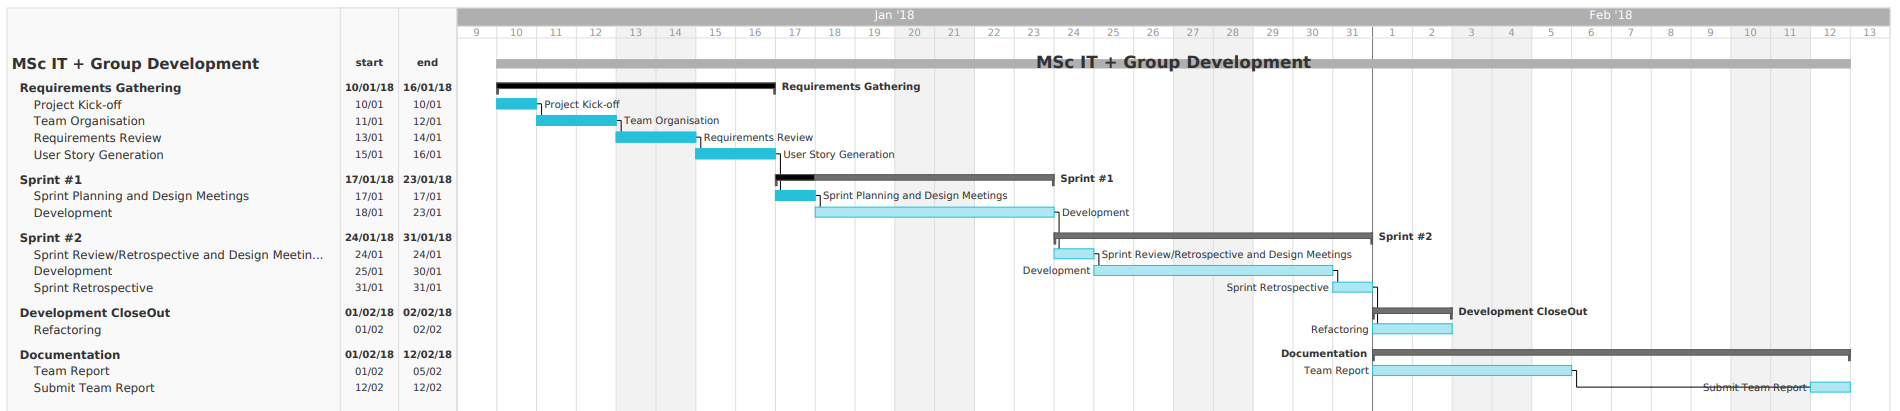
\includegraphics[scale=0.35, angle=90]{initial_project_plan}
	\captionof{figure}{Initial Project Plan}
	\label{figure:initial_project_plan}
\end{center}


\newpage
\subsection{System Design Meeting}

\momtoptable
{Wed 17-Jan 2018 (Week 2)}
{Slack}
{Christopher Bellingham}
{Ioannis Athanasiadis [IA]\newline
Christopher Bellingham [CB]\newline
Joseph Doogan [JD]\newline
Pavlos Evangelidis [PE]\newline
Torquil MacLeod [TM]}
{-}

\begin{momitems}
	% Item, Details, Resp., Due.
	\momitem
	{1}
	{CB provided a candidate architecture diagram (Figure \ref{figure:initial_architecture}), outlining use of an MVC architecture, with a data persistence layer. CB proposed use of the Observer Pattern as a means of reducing coupling between MVC layers.}
	{INFO}
	{INFO}

	\momitem
	{2}
	{Use of the Observer Pattern was identified as a risk, since no team member has experience with this. CB will outline how this would work by providing an example of a simple implementation.}
	{CB}
	{Wed 17-Jan}

	\momitem
	{3}
	{Prior to the meeting, each team member had submitted class diagrams to enable discussion on needed class structures. Each submission was reviewed, and it was noted that a lot of commonality exists across proposed classes (typically Game, Player and Card classes).}
	{INFO}
	{INFO}

	\momitem
	{4}
	{CB provided detailed UML covering full system (Figure \ref{figure:initial_uml}). It is understood that online mode can hook into key Game functionality via game's available public methods, and online components can be notified of game state changes via the Observer mechanism. The approach as depicted was agreed to be a reasonable solution, and was selected as a basis for overall design.}
	{INFO}
	{INFO}

	\momitem
	{5}
	{CB provided detailed sequence diagram covering logical flow for command line mode (Figure \ref{figure:initial_sequence_diagram}). This may be used as a reference during development.}
	{INFO}
	{INFO}

	\momitem
	{6}
	{User stories allocated to team from Appendix \ref{appendix:user_stories_command_line} to allow development to commence.}
	{INFO}
	{INFO}
\end{momitems}

\begin{center}
	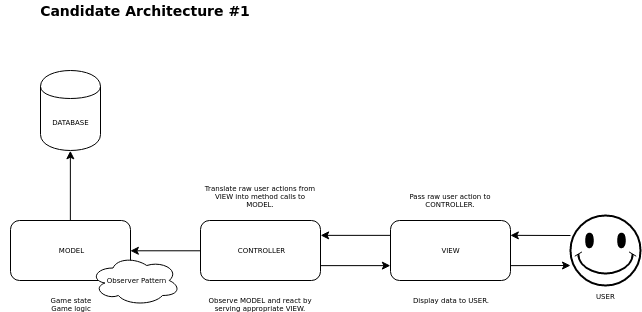
\includegraphics[scale=0.7]{initial_architecture}
	\captionof{figure}{Proposed Architecture}
	\label{figure:initial_architecture}
\end{center}

\begin{center}
	\missingfigure{Include UML with Joe's updates.}
	\captionof{figure}{Proposed UML}
	\label{figure:initial_uml}
\end{center}

\begin{center}
	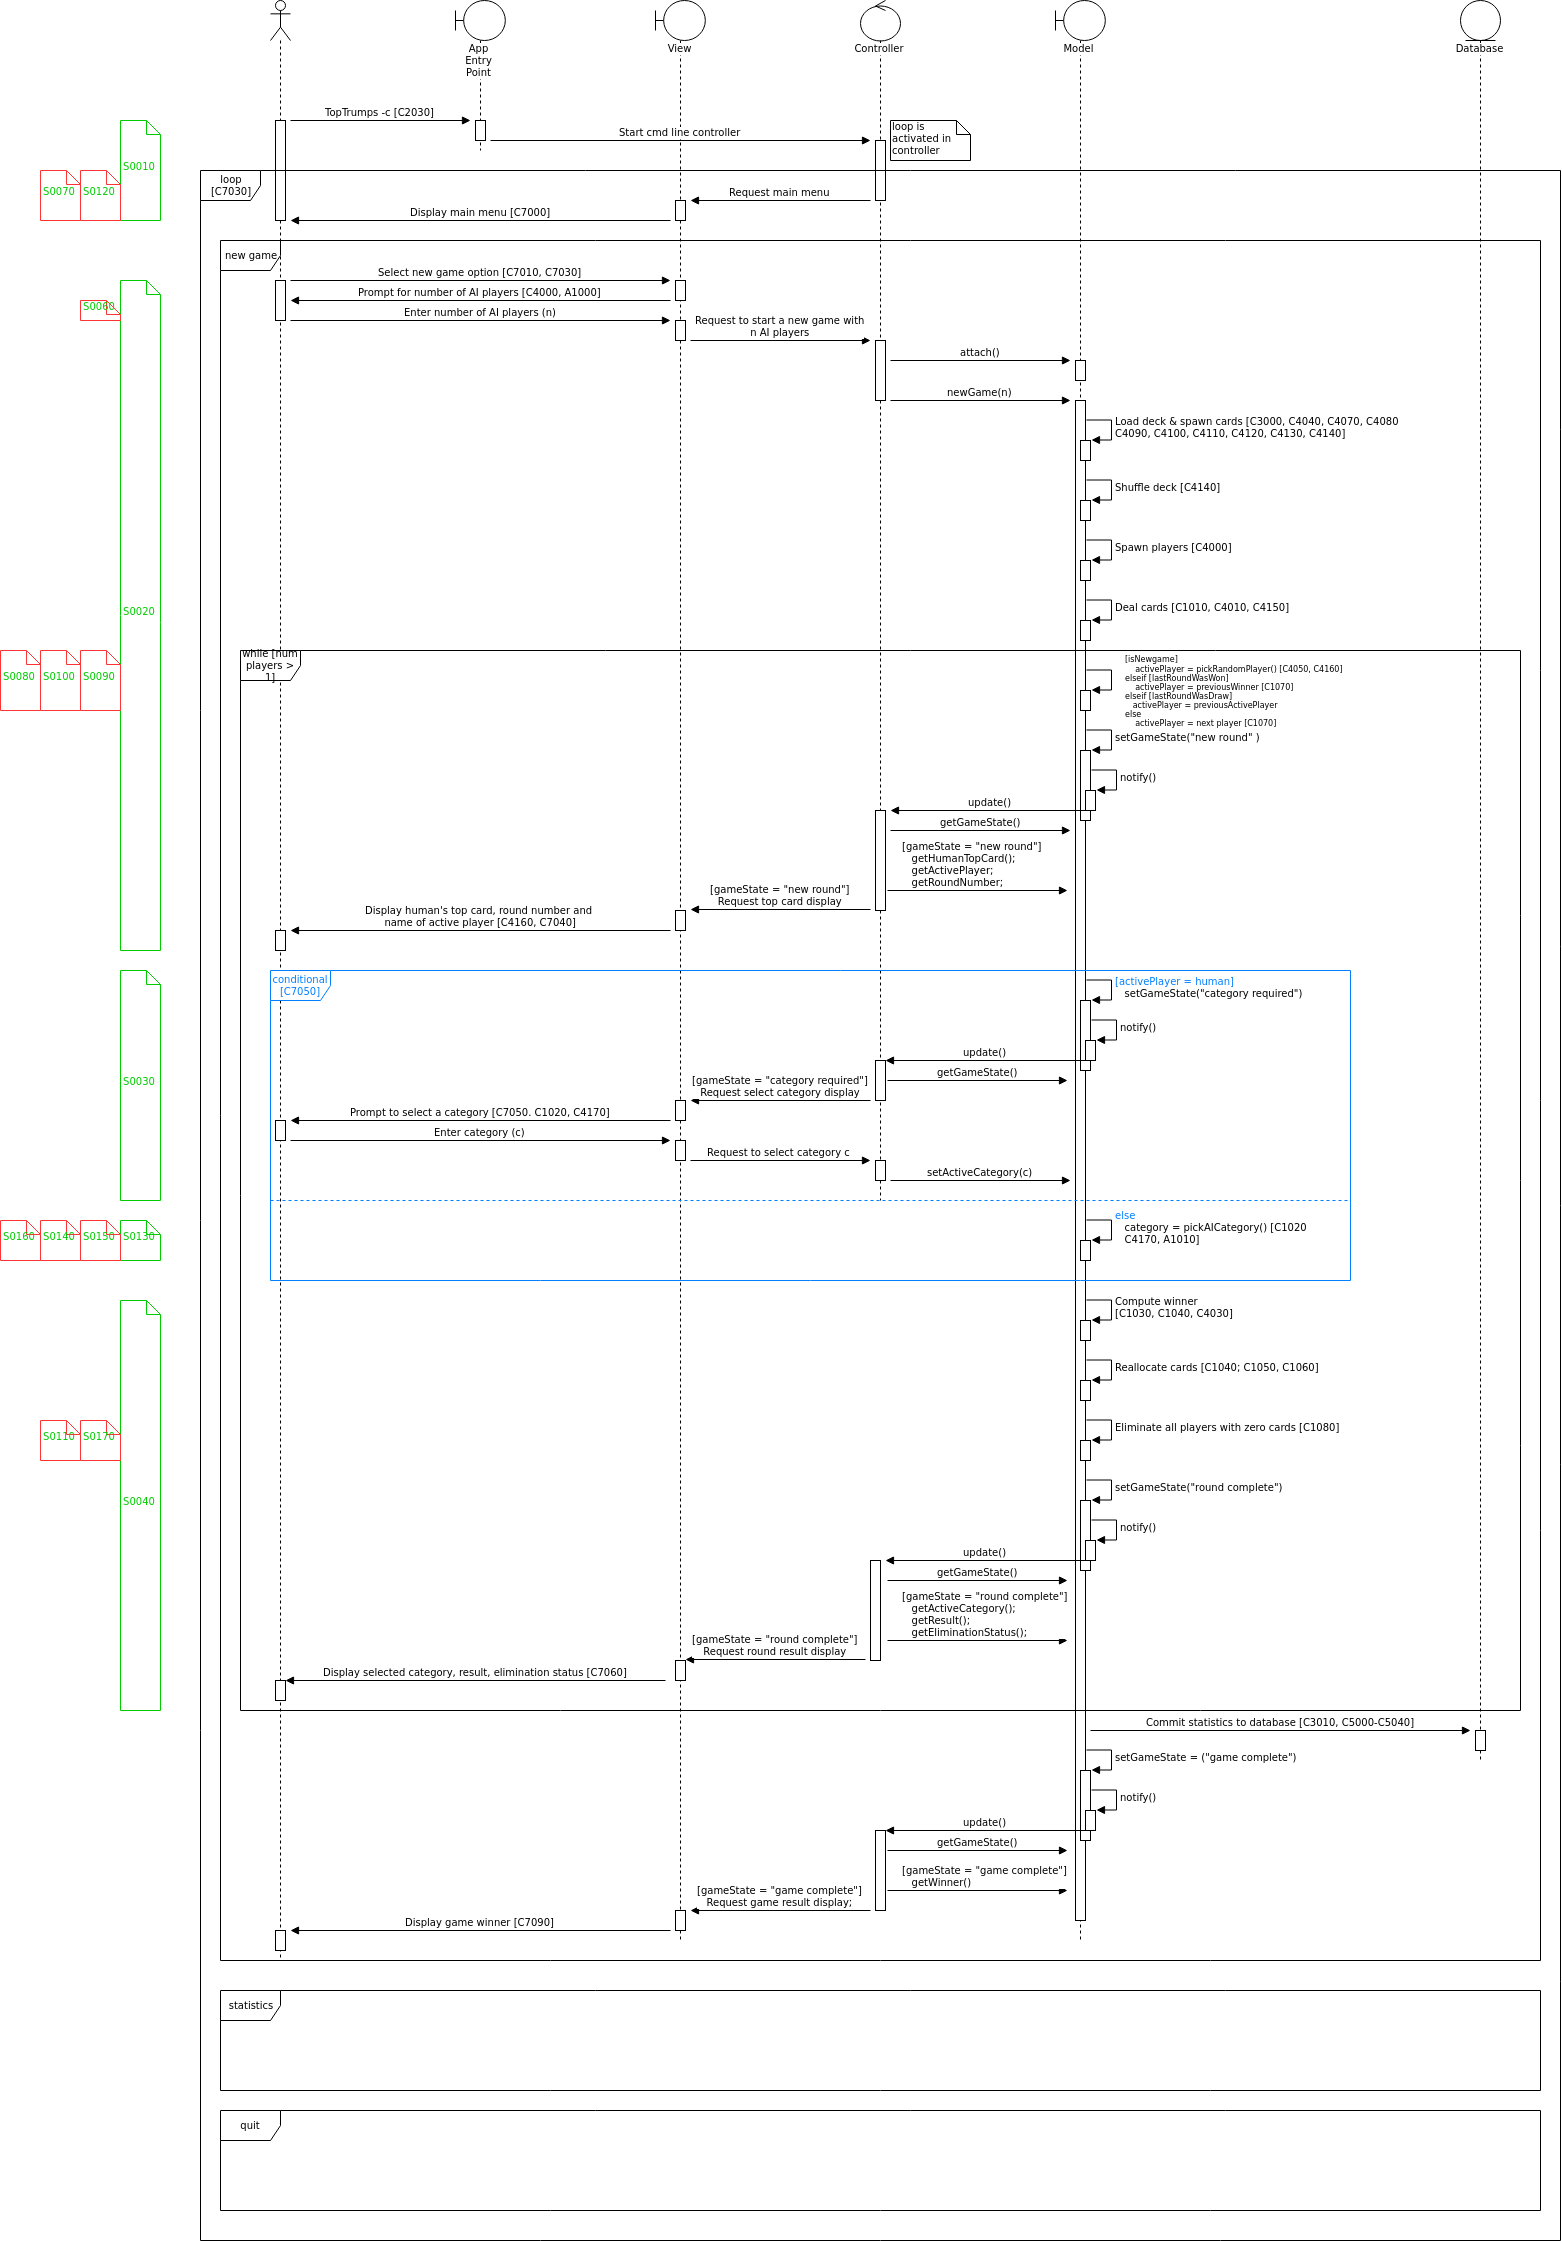
\includegraphics[scale=0.25]{initial_sequence_diagram}
	\captionof{figure}{Proposed Logical Flow}
	\label{figure:initial_sequence_diagram}
\end{center}


\newpage
\subsection{Sprint Review/Planning Meeting}
\label{appendix:sprint2_planning_meeting}

\momtoptable
{Wed 24-Jan 2018 (Week 3)}
{Slack}
{Christopher Bellingham}
{Ioannis Athanasiadis [IA]\newline
Christopher Bellingham [CB]\newline
Joseph Doogan [JD]\newline
Pavlos Evangelidis [PE]\newline
Torquil MacLeod [TM]}
{-}

\begin{momitems}
	% Item, Details, Resp., Due.
	\momitem
	{}
	{}
	{}
	{}
\end{momitems}


\newpage
\subsection{Sprint Review/Planning Meeting}
\label{appendix:sprint3_planning_meeting}

\momtoptable
{Wed 31-Jan 2018 (Week 4)}
{Slack}
{Christopher Bellingham}
{Ioannis Athanasiadis [IA]\newline
Christopher Bellingham [CB]\newline
Joseph Doogan [JD]\newline
Pavlos Evangelidis [PE]\newline
Torquil MacLeod [TM]}
{-}

\begin{momitems}
	% Item, Details, Resp., Due.
	\momitem
	{}
	{}
	{}
	{}
\end{momitems}
	\newpage
\section{Customer Specification}
\label{appendix:customer_specification}

\newcommand{\creq}[1]{
    [\textbf{C\arabic{cReqNum}: #1}]%
    %\appto{\creqHook}{\arabic{cReqNum} #1 }%
    \addtocounter{cReqNum}{10}%
}

\newcommand{\areq}[1]{
    [\textbf{A\arabic{aReqNum}: #1}]%
    %\appto{\creqHook}{\arabic{cReqNum} #1 }%
    \addtocounter{aReqNum}{10}%
}

\subsection{Purpose}

This appendix captures the foundational requirements of the system.

Section \ref{contract} is quoted verbatim from Assignment Specification ITSD2018-TaskDocument.
Requirements within are identified in \textbf{bold} and given a unique requirement ID, used for cross-referencing with User Stories.

\subsection{Customer Specification} \label{contract}
\newcounter{cReqNum}
\setcounter{cReqNum}{1000}
\subsubsection{Context}
Top Trumps is a simple card game in which decks of cards are based on a theme.
For example, race cars, dinosaurs, and even TV shows like ``The Simpsons''.
Within a deck each card represents an entity within that topic (e.g. T-Rex for dinosaurs or Bart Simpson for the Simpsons).
Within a deck each card has the same list of characteristics.
For example, dinosaurs can have a height, weight, length, ferocity, and intelligence.
Each card has a value for each characteristic of the deck.
The objective of the game is to ``trump'' your opponent by selecting a category (e.g. intelligence) and having a ``better'' value for your card than the opponent does in their current card.

Gameplay is as follows:
\begin{itemize}
    \item
    \creq{There must be at least two players}.
    \creq{The deck of cards is divided between the players}.
    \creq{The first player takes their topmost card and selects a characteristic}.
    \creq{The value of that characteristic is compared against the value for the same characteristic in the other players' top card}.
    \creq{The player with the best value for that characteristic wins the round and the winner takes all the cards from that round (including their own) and places them at the back of their deck}.
    \creq{If there is a draw the cards from the round are placed in a new communal pile and a new characteristic is selected by the same player from the next card}.
    \creq{The winner then takes the cards from the round and any in the communal pile}.
    \creq{The winner of a round maintains the choice of category until they lose, then the choice moves to the next player}.
    \creq{Players lose the game when they have no cards left; the player left with all the cards is the winner of the game}.
\end{itemize}

\subsubsection{Aim}
\setcounter{cReqNum}{2000}
The aim is to build a computer program to allow a user to play top trumps against one or more AI opponents given a deck.
\creq{The program should have two modes}:
\begin{itemize}
    \item
    \creq{Command Line Mode: The game is played only through command line input and output}.
    \creq{In this mode, only one game can be played at a time}.
    \creq{This mode should be selected via a ‘-c’ flag when starting the program}:
    o java -jar TopTrumps.jar -c
    \item
    \creq{Online Mode: The game should be hosted as a web service, comprised of a REST API that provides remote access to the core game functionality and one or more web-pages that enable a user to play the game}.
    \creq{In this mode, multiple users should be able to play the game concurrently (e.g. in different Web browser tabs)}. 
    \creq{This mode should be selected via a ‘-o’ flag when starting the program}:
    o java -jar TopTrumps.jar -o
\end{itemize}

\subsubsection{Functionality}
\setcounter{cReqNum}{3000}
In both modes, the program needs to:
\begin{itemize}
    \item
    \creq{Enable a user to play a game of top trumps with a deck that was loaded in when the program started}.
    \item
    \creq{Store the results of past games played in a database as well as visualize that information to the user on-demand}.
\end{itemize}

In command line mode only:
\begin{itemize}
    \item
    \creq{Write a ‘test log’ to file that contains snapshots of the program’s state as it runs}.
\end{itemize}

We discuss each of these requirements in more detail below:

\paragraph{Playing Top Trumps}
\setcounter{cReqNum}{4000}
The program should implement the top trumps game as described in the Context section above. You can make the following assumptions to simplify the implementation. Do not add additional unnecessary functionality. This is ‘gold-plating’ and will not result in a better grade. If in doubt, consult the course co-ordinator.

\begin{itemize}
    \item
    \creq{There should be one human player and up to 4 computer players (AIs)}.
    \item
    \creq{If a deck does not divide equally between the players, then some players may have less cards.
    For example, if there are 3 players and 40 cards, then two players receive 13 cards and one player receives 14}.
    \item
    \creq{A deck has 5 criteria and the criteria are always positive integers between 1 and 50 (inclusive)}.
    \item
    \creq{A higher number is always better for any given characteristic}.
    \item
    \creq{There are 40 cards in a deck.txt file}.
    \item
    \creq{The first player should be selected at random}.
    \item
    \creq{A draw won't continue until the point where there are only cards in the communal pile – you do not need to deal with this programmatically, just assume that should this happen you are not expected to deal with it}.
\end{itemize}

\creq{The deck we will be using is stored in a text file called 'StarCitizenDeck.txt'}.
\creq{The first line of the text file should contain a list of the categories in the deck, separated by a space}.
\creq{All decks should have a 'description' category to label the individual cards}.
\creq{A description within a deck can be assumed to be unique and a single word}.
\creq{The subsequent lines contain details of one card}.
\creq{You can assume the order of the categories from the first line align with 3 the values provided for the cards and that all cards have a value for all categories in a deck}.
\creq{You can assume that all categories are single words}.

For example, in a dinosaur deck (numbers bear no resemblance to reality):

\begin{verbatim}
    description height weight length ferocity intelligence
    TRex 6 6 12 9 9
    Stegosaurus 4 3 8 1 8
    Brachiosaurus 12 8 16 2 6
    Velociraptor 3 5 5 12 10
    Carnotaurus 5 6 7 9 8
    Iguanodon 2 2 3 1 9
    Megalosaurus 9 9 8 6 9
    Oviraptor 8 7 4 3 2
    Parasaurolophus 7 7 1 3 4
    Ornithomimus 10 9 8 7 5
    Protoceratops 9 5 4 7 10
    Riojasaurus 6 1 4 7 7
    Saurolophus 7 1 10 7 8
    Styracosaurus 7 3 4 1 1
    Xiaosaurus 10 6 5 7 2
\end{verbatim}

and so forth – the star citizen-based deck is provided with the Template Package that can be downloaded from Moodle.

\creq{The program must first load all card details from the deck and shuffle them (randomly order them)}.
\creq{The program should then deal the cards between the players}.
\creq{The user should then be shown the detail from their top card (note there is no need to visualise this in a complex manner, the card details can be shown in text) and the first player is randomly selected}.
\creq{If the player is an AI player it should select a category for play, if the user is the first player they should be allowed to select a category to play the round}.
\creq{The game play should then proceed as detailed in the section Context}.

\paragraph{Persistent Game Data}
\setcounter{cReqNum}{5000}
\creq{Upon completion of the game, the user should automatically write the following information about the game play to a database}:
\begin{itemize}
    \item
    \creq{How many draws were there?}
    \item
    \creq{Who won the game?}
    \item
    \creq{How many rounds were played in the game?}
    \item
    \creq{How many rounds did each player win?}
\end{itemize}

You should select one team member’s database on the yacata server, from the Database Theory and Applications course, to write to.
\creq{It is important you do not remove the username and password from the final code, as this allows us to test the software}.
You should also provide details of this database (username, database name and password) in the report.

\creq{There should also be possible, so long as a game isn't currently in progress, for the user to connect to the database and get information about previous games}. 
This should include the following:
\begin{itemize}
    \item
    \creq{Number of games played overall}.
    \item
    \creq{How many times the computer has won}.
    \item
    \creq{How many times the human has won}.
    \item
    \creq{The average number of draws}.
    \item
    \creq{The largest number of rounds played in a single game}.
    \item
    \creq{These values should be calculated using SQL}.
\end{itemize}

\paragraph{Test Log}
\setcounter{cReqNum}{6000}
In addition to the functionality described above, you should implement the following to allow for program debugging when in command line mode only. 
\creq{When the program is started, if a ‘-t’ flag is set on the command line, then the program should write out an extensive log of its operation to a ‘toptrumps.log’ file in the same directory as the program is run}, e.g.: java -jar TopTrumps.jar -c -t

\creq{If a toptrumps.log file already exists, your program should overwrite that file}.
\creq{Your program should print the following information to that file, separated by a line containing dashes at the appropriate times as mentioned below}:
\begin{itemize}
    \item
    \creq{The contents of the complete deck once it has been read in and constructed}.
    \item
    \creq{The contents of the complete deck after it has been shuffled}.
    \item
    \creq{The contents of the user’s deck and the computer’s deck(s) once they have been allocated.
    Be sure to indicate which the user’s deck is and which the computer’s deck(s) is}.
    \item
    \creq{The contents of the communal pile when cards are added or removed from it}.
    \item
    \creq{The contents of the current cards in play (the cards from the top of the user’s deck and the computer’s deck(s))}.
    \item
    \creq{The category selected and corresponding values when a user or computer selects a category}.
    \item
    \creq{The contents of each deck after a round}.
    \item
    \creq{The winner of the game}.
\end{itemize}

\paragraph{Command Line Mode}
\setcounter{cReqNum}{7000}
\creq{When started in command line mode, the program should ask the user whether they want to see the statistics of past games (see the Persistent Game Data section) or whether they want to play a game}.
\creq{The user’s choice should be obtained from standard in (System.in)}. 
\creq{If they select to see statistics of past games, the program should print the associated statistics to standard out (System.out) and then ask the same question again}.
\creq{If they select to play a game, a game instance should be started, and the core game loop initialized}.
\creq{For each round, the round number, the name of the active player and the card drawn by the player should be printed to standard out}.
\creq{If the user is the active player, then it should ask the player to select a category, and obtain the user’s choice from standard in, otherwise the AI player should select a category}.
\creq{The program should then print to standard out the selected category, who won (or whether it was a draw), the winning card and whether the player has been eliminated (they have no cards left)}.
\creq{Rounds should continue to be played until a winner is determined (only one player has cards left)}.
\creq{Once the user has been eliminated, the remaining rounds should be completed automatically (without user input)}.
\creq{At the end of the game, the overall winner should be printed, and the Persistent Game statistics should be updated}.
\creq{The user should then be asked if they want to print the statistics of past games or play another game}.
\creq{An example of the command line output for the program is provided in the ‘CLI.example.txt’ file on Moodle}.

\paragraph{Online Mode}
\setcounter{cReqNum}{8000}
Online mode is an extension to the command line mode that provides a version of the game that users can play through their Web browser. 
A Web application has two main components. 
First, a back-end Application Programming Interface (API) that provides remote access to the game functionalities (e.g. starting a new game, drawing cards or getting players/cards for display). 
Second, one or more webpages that use the back-end API to enable the user to play the game.
In this case, each web page should be comprised of HTML elements that are displayed and Javascript functions that connect to the API.

The webpage design is down to you, but it should display the following:
\begin{itemize}
    \item
    \creq{Upon loading the web page, the user should be presented the option to view overall game statistics (as detailed previously), or play a single game}.
    \item
    \creq{During game play, the GUI should display the contents of the user’s top card and, when they are the active player, allow the user to select a category to play against the computer}.
    \item
    \creq{The GUI should clearly indicate who’s turn it currently is, and only allow the user to select a category when it is their turn}.
    \item
    \creq{Once the category has been selected for a round and the values compared, the GUI should display the values of the category for each player and highlight who won the round}.
    \item
    \creq{If a draw should occur, the user should be notified of this}.
    \item
    \creq{The GUI should contain an indication of how many cards are in the communal pile}.
    \item
    \creq{The GUI should contain an indication of how many cards are left in the user’s deck and in the computer’s deck(s)}.
    \item
    \creq{When the round played results in the game finishing, an indication of the overall winner should be presented to the user along with an option to update the database with the statistics of the game as previously described}.
\end{itemize}

	\newpage
\section{Final User Stories}
\label{appendix:user_stories}

\subsection{Sprint \#1: Command Line Mode} 
\label{appendix:user_stories_command_line}
\bigskip

% ---------------------------------

\begin{card}{green}
{S0010}
{Must Have}
{Est: 1}
{Act: 1}
As a Human Player, I want to start the program in command line mode, so that I can either play a new game or see statistics of previous games.
\end{card}

\begin{card}{blue}
{S0010}{}{}{}
BOB can start the program in CL and he is presented with a question of whether he wants to play a new game, view statistics or quit. 
The question asks Bob to enter ``1'' for a new game, ``2'' for viewing the stats, ``3'' to quit the game, and he must ``press enter'' to submit his choice. Acceptance tests: Try to press enter with empty string. 
Try with a random number other than ``1'', ``2'' or ``3'' Try with correct numbers.
\end{card}

% ---------------------------------

\newpage

\begin{card}{green}
{S0020}
{Must Have}
{Est: 2}
{Act: 2}
As a Human Player, I want to start a new game, so that the first active player can select a category.
\end{card}

\begin{card}{blue}
{S0020}{}{}{}
Test that deck is loaded. 
Test that deck is shuffled. 
Test that correct number of players are created. 
Test that players are dealt the correct number of cards. 
Test that one player is made the active player. 
Test that correct output is provided by standard out.
\end{card}

% ---------------------------------

\newpage

\begin{card}{green}
{S0030}
{Must Have}
{Est: 1}
{Act: 2}
As a Human Player who is selected as the active player, I want to select a category, so that the game can check the outcome of the round.
\end{card}

\begin{card}{blue}
{S0030}{}{}{}
After the current round finishes, BOB can check the screen to find out who the winner was. 
The format is ``X wins this round'' with X being BOB or the AI player. 
The category values for each player are presented on the screen. 
Acceptance Tests: Play a round and check that the correct category values are shown for each player. 
Check that the correct player wins each time. Check that draw takes place if there are multiple highest cards. 
Check that correct player becomes/remains active player for next round. 
Check whether there is a message at the end specifying the winner.
\end{card}

% ---------------------------------

\newpage

\begin{card}{green}
{S0040}
{Must Have}
{Est: 1}
{Act: 2}
As a Human Player I want to know the outcome of the round, so that the game can progress to the next round.
\end{card}

\begin{card}{blue}
{S0040}{}{}{}
BOB will know if it is his or the opponents round without having to do anything further.
Tests: Check that after each round there is an output mentioning the winner. 
Check that user can continue to progress to new rounds even if eliminated.
\end{card}

% ---------------------------------

\newpage

\begin{card}{green}
{S0050}
{Must Have}
{Est: 1}
{Act: 1}
As a human player I want to choose to record game log information in a file when I start a game in command line mode.
\end{card}

\begin{card}{blue}
{S0050}{}{}{}
BOB can navigate to the game folder and see the game log. 
(Not sure if the user has the option NOT to log the game information) 
Acceptance Tests: Initiate a game and set -t flag in the CL. 
After the game finishes check that there exists a log file in the game directory, named topTrumps.log. 
Write a test log file with known content. 
RE-run the game and check that the original file is overwritten with the correct content. 
Check the content of the file as per C6030- C6100 requirements.
\end{card}

% ---------------------------------

\newpage

\begin{card}{green}
{S0130}
{Must Have}
{Est: 1}
{Act: 2}
As a Human Player, when not the active player for a round, I want the active AI player to select a single category which has the highest or joint highest value for their topmost card.
\end{card}

\begin{card}{blue}
{S0130}{}{}{}
While developing, have the system.out print all the values for the AI player, i.e. the contents of their top most card. 
Upon selecting a category, have a system.out for the category selected and the value. 
Compare with the contents of the whole card to make sure that the highest value category is always selected by the AI player.
\end{card}

% ---------------------------------

\newpage

\begin{card}{green}
{S0180}
{Must Have}
{Est: 2}
{Act: 2}
Bob and Lilly are really into statistics and they want to keep track of the game stats after a game ends. 
As experienced players they want to know how many draws were in the game, how many rounds were played, how many rounds were won by each player (with clear indication) and who won the game. 
They don't want to press anything for this procedure, it must be automated.
\end{card}

\begin{card}{blue}
{S0180}{}{}{}
Query the Database to make sure everything has been recorded.
\end{card}

% ---------------------------------

\newpage
\subsection{Sprint \#2: Online Mode}
\label{appendix:user_stories_online}
\bigskip

\begin{card}{green}
{S0190}
{Must Have}
{Est: 1}
{Act: 1}
Lilly, is known for her attitude of succeeding on everything, so she always watch her performance before starting a game (access the DB before a game starts). 
She wants to see the number of games played overall, how many times a human won and how many the ``AI'', the average draws per game, the largest number of rounds played in a game.
\end{card}

\begin{card}{blue}
{S0190}{}{}{}
?
\end{card}

% ---------------------------------

\newpage

\begin{card}{green}
{S0200}
{Must Have}
{Est: \st{1} 2}
{Act: 2}
As a Human Player, I want to start the game in the online mode by using an -o flag either in terminal.  
I want to be able to start a new game in different tabs and play different games concurrently with 1-4 opponents. 
After I run the command in terminal, I can open a browser and initialise a game by typing in http://localhost:7777/toptrumps.
\end{card}

\begin{card}{blue}
{S0200}{}{}{}
Try in terminal with -o flag and check for errors. 
If no errors occur, open browser and type in the http.
Check multiple tabs to check that the initial selection screen is active Check that the selection screen contains buttons for new game and statistics.
Click on the Start Game button and check that the browser displays the correct number of game. 
Check that the human player is always present and that the AI players are present and not more than four. 
If number of AI players is not selected randomly, check that my input corresponds to the number of AI players on screen.
\end{card}

% ---------------------------------

\newpage

\begin{card}{green}
{S0210}
{Must Have}
{Est: 1}
{Act: 1}
As a Human Player, I want to be able to access the DB to view statistics upon clicking the Statistics button on the selection screen.
This has the same functionality as in the Command Line mode as described in [S0180].
The difference is the way I will access this functionality.
\end{card}

\begin{card}{blue}
{S0210}{}{}{}
Check that the Statistics button is responsive. 
Check that all games are stores to the DB, I.e all instances as represented by different tabs.
\end{card}

% ---------------------------------

\newpage

\begin{card}{green}
{S0220}
{Must Have}
{Est: \st{1} 2}
{Act: (incomplete)}
As a Human Player, I want to be able to see that the game has actually started, and be guided through the steps of what I need to do next. 
I want to be able to have access on the game information that allow me to navigate through it, and be presented with my options if I am the active player, or have a visual on the storyline if an AI is the active player.
\end{card}

\begin{card}{blue}
{S0220}{}{}{}
After clicking on the new game button check that the screen shows: Confirmation that the game has started, by showing for example ``Deck has been shuffled and dealt''.
The round number I am currently playing Who the active player is.
Check that I have the number of cards I have in hand, either on the card, or somewhere else on screen.
My topmost card with the characteristics' values.
A button that allows me to proceed to the next step. 
That is, to select my category if I am the active player or make the AI plaeyer select his. 
Check that if I am not the active player I do not have the option to select my category.
\end{card}

% ---------------------------------

\newpage

\begin{card}{green}
{S0230}
{Must Have}
{Est: \st{1} 2}
{Act: (incomplete)}
As a Human Player, and after I have selected to proceed with the game after selecting the button as described by S0220, I want to trigger the current round.
I want to be able to select my category as an active player, or ``notify'' the AI player that he needs to do the same, and in the end I would like to know the outcome of the round.
\end{card}

\begin{card}{blue}
{S0230}{}{}{}
If I am the active player: Check that the button makes me select a category by poping a drop down menu or similar. 
Check that selecting my category the game proceeds to next step If I am not the active player. 
Check that the game continies by having the AI player selecting category.
In both cases: After selection, check that I have the option to go to the next step, I.e. show the winner After the category selection, check that all cards with their values are visible on screen and that the winner is mentioned. 
Check that the same winner has the privilege of selecting the new category Check that the number of available cards in hand have been recalculated.
\end{card}

% ---------------------------------

\newpage

\begin{card}{green}
{S0240}
{Must Have}
{Est: 1}
{Act: (incomplete)}
As a Human Player, I want to have access to the game information if a draw has occurred. 
That includes to be aware that the outcome was a draw and the size of the communal deck. 
I want to be able to re-select if I was the winner of the previous round. 
\end{card}

\begin{card}{blue}
{S0240}{}{}{}
Check that in the case of a draw, the screen shows that clearly. 
Next check that there is an indication of the number of cards in the communal pile Check that a button is present, allowing me to order the game to proceed to the next round. 
Check that the round number has increased by 1 after the draw and after I have selected to go on. 
Check that the category selector from previous round is the current selector. 
In the first winning case, display the number of cards in communal pile to make sure it is reset.
\end{card}

% ---------------------------------

\newpage

\begin{card}{green}
{S0250}
{Must Have}
{Est: 1}
{Act: (incomplete)}
As a Human Player, I want to know who the overall winner was.
\end{card}

\begin{card}{blue}
{S0250}{}{}{}
Check that when the last round is finished, the name of the winner is shown. Make sure there is an option to return me to the selection menu, from where I can access the DB or play new game.
\end{card}

% ---------------------------------

\newpage
\subsection{Sprint \#3: Online Mode (Additional)}
\label{appendix:user_stories_online_additional}
\bigskip

% ---------------------------------

\begin{card}{green}
{S0220}
{Must Have}
{Est: 4}
{Act: 4}
As a Human Player, I want to be able to see that the game has actually started, and be guided through the steps of what I need to do next. 
I want to be able to have access on the game information that allow me to navigate through it, and be presented with my options if I am the active player, or have a visual on the storyline if an AI is the active player.
\end{card}

\begin{card}{blue}
{S0220}{}{}{}
After clicking on the new game button check that the screen shows: Confirmation that the game has started, by showing for example ``Deck has been shuffled and dealt''.
The round number I am currently playing Who the active player is.
Check that I have the number of cards I have in hand, either on the card, or somewhere else on screen.
My topmost card with the characteristics' values.
A button that allows me to proceed to the next step. 
That is, to select my category if I am the active player or make the AI plaeyer select his. 
Check that if I am not the active player I do not have the option to select my category.
\end{card}

% ---------------------------------

\newpage

\begin{card}{green}
{S0230}
{Must Have}
{Est: 4}
{Act: 4}
As a Human Player, and after I have selected to proceed with the game after selecting the button as described by S0220, I want to trigger the current round.
I want to be able to select my category as an active player, or ``notify'' the AI player that he needs to do the same, and in the end I would like to know the outcome of the round.
\end{card}

\begin{card}{blue}
{S0230}{}{}{}
If I am the active player: Check that the button makes me select a category by poping a drop down menu or similar. 
Check that selecting my category the game proceeds to next step If I am not the active player. 
Check that the game continies by having the AI player selecting category.
In both cases: After selection, check that I have the option to go to the next step, I.e. show the winner After the category selection, check that all cards with their values are visible on screen and that the winner is mentioned. 
Check that the same winner has the privilege of selecting the new category Check that the number of available cards in hand have been recalculated.
\end{card}

% ---------------------------------

\newpage

\begin{card}{green}
{S0240}
{Must Have}
{Est: 2}
{Act: 2}
As a Human Player, I want to have access to the game information if a draw has occurred. 
That includes to be aware that the outcome was a draw and the size of the communal deck. 
I want to be able to re-select if I was the winner of the previous round. 
\end{card}

\begin{card}{blue}
{S0240}{}{}{}
Check that in the case of a draw, the screen shows that clearly. 
Next check that there is an indication of the number of cards in the communal pile Check that a button is present, allowing me to order the game to proceed to the next round. 
Check that the round number has increased by 1 after the draw and after I have selected to go on. 
Check that the category selector from previous round is the current selector. 
In the first winning case, display the number of cards in communal pile to make sure it is reset.
\end{card}

% ---------------------------------

\newpage

\begin{card}{green}
{S0250}
{Must Have}
{Est: 1}
{Act: 1}
As a Human Player, I want to know who the overall winner was.
\end{card}

\begin{card}{blue}
{S0250}{}{}{}
Check that when the last round is finished, the name of the winner is shown. Make sure there is a button to return me to the selection screen, from where I can access the DB or play new game.
\end{card}

% \begin{card}{green}
% {S?}
% {?}
% {Est: ?}
% {Act: ?}
% ?
% \end{card}

% \begin{card}{blue}
% {S?}{}{}{}
% ?
% \end{card}
	\newpage
\section{Screenshots}
\label{appendix:screenshots}

\begin{center}
	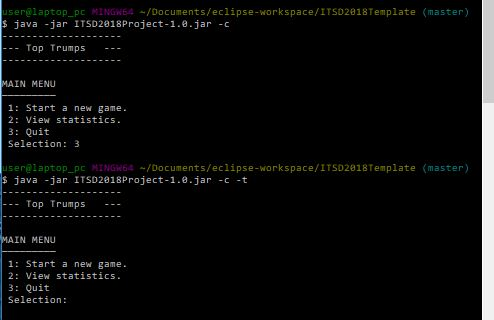
\includegraphics[width=0.8\textwidth]{S0010_GameInit}
	\captionof{figure}{Game Initialisation.}
	\label{figure:gameInit_true}
\end{center}
\begin{center}
	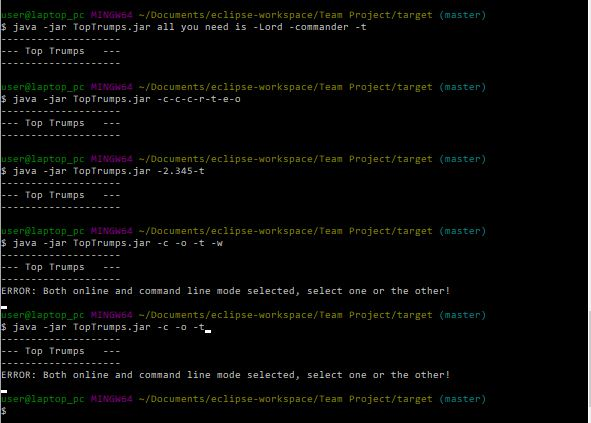
\includegraphics[width=0.8\textwidth]{S0010_GameInitAnti}
	\captionof{figure}{Game Initialisation with wrong flag.}
	\label{figure:gameInit_false}
\end{center}
\begin{center}
	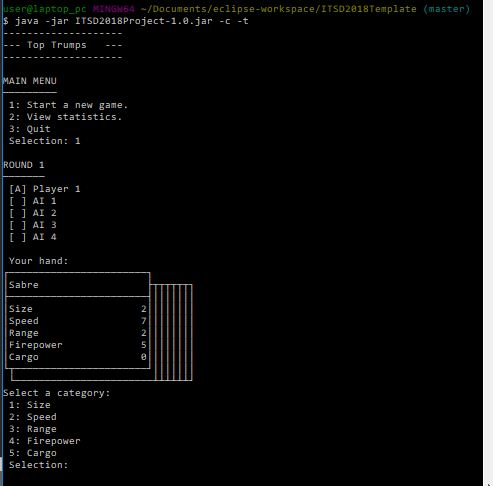
\includegraphics[width=0.8\textwidth]{S0010_MainMenu}
	\captionof{figure}{Main Menu with correct integer.}
	\label{figure:mainMenu_true}
\end{center}
\begin{center}
	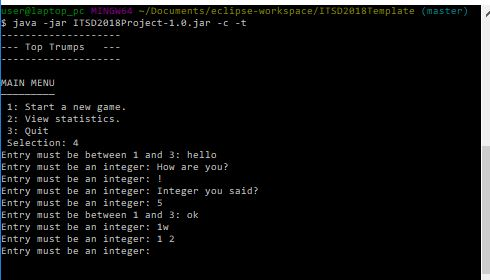
\includegraphics[width=0.8\textwidth]{S0010_MainMenuAnti}
	\captionof{figure}{Main Menu with incorrect integer.}
	\label{figure:mainMenu_false}
\end{center}
\begin{center}
	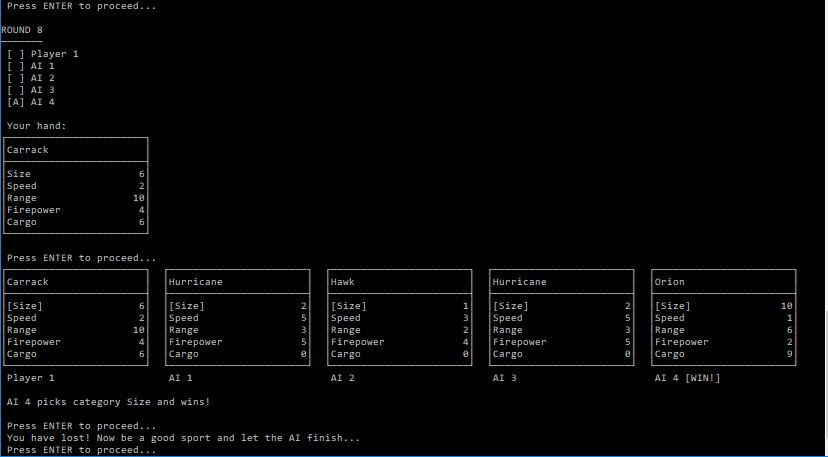
\includegraphics[width=0.8\textwidth]{S0030_S0040_RoundInfo}
	\captionof{figure}{Round information and human player is eliminated.}
	\label{figure:cmd_winner}
\end{center}
\begin{center}
	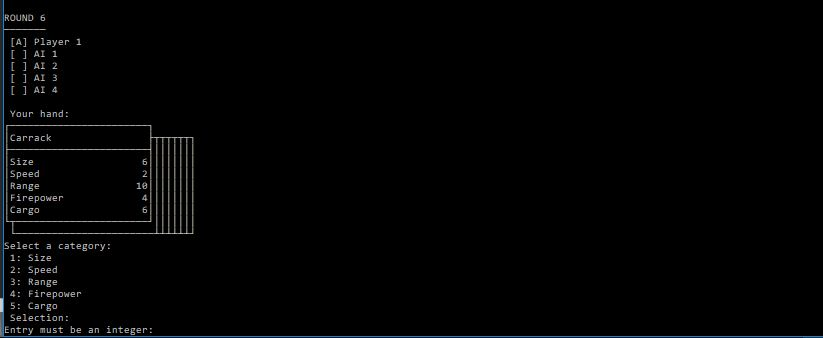
\includegraphics[width=0.8\textwidth]{S0030_HumanActive}
	\captionof{figure}{Human player is active player and has to select a category.}
	\label{figure:cmd_play}
\end{center}
\begin{center}
	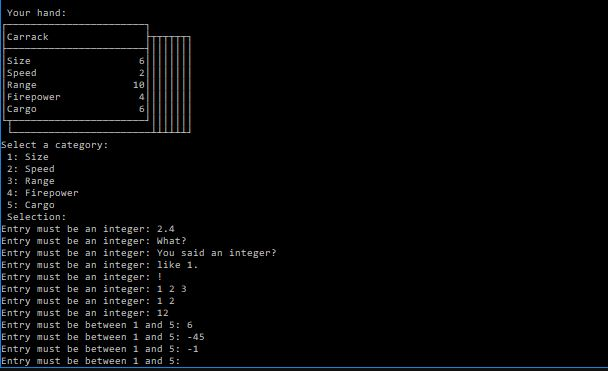
\includegraphics[width=0.8\textwidth]{S0030_WrongInput}
	\captionof{figure}{Human player is active player and enters wrong integer number.}
	\label{figure:falseInput}
\end{center}
\begin{center}
	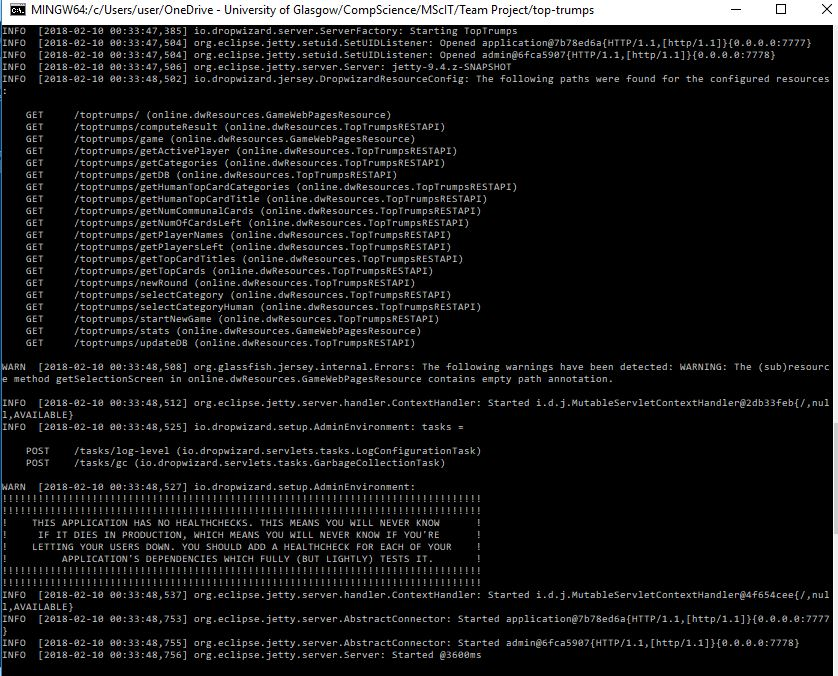
\includegraphics[width=0.8\textwidth]{S0200_OnlineMode}
	\captionof{figure}{Initialise online game mode.}
	\label{figure:onlineMode}
\end{center}
\begin{center}
	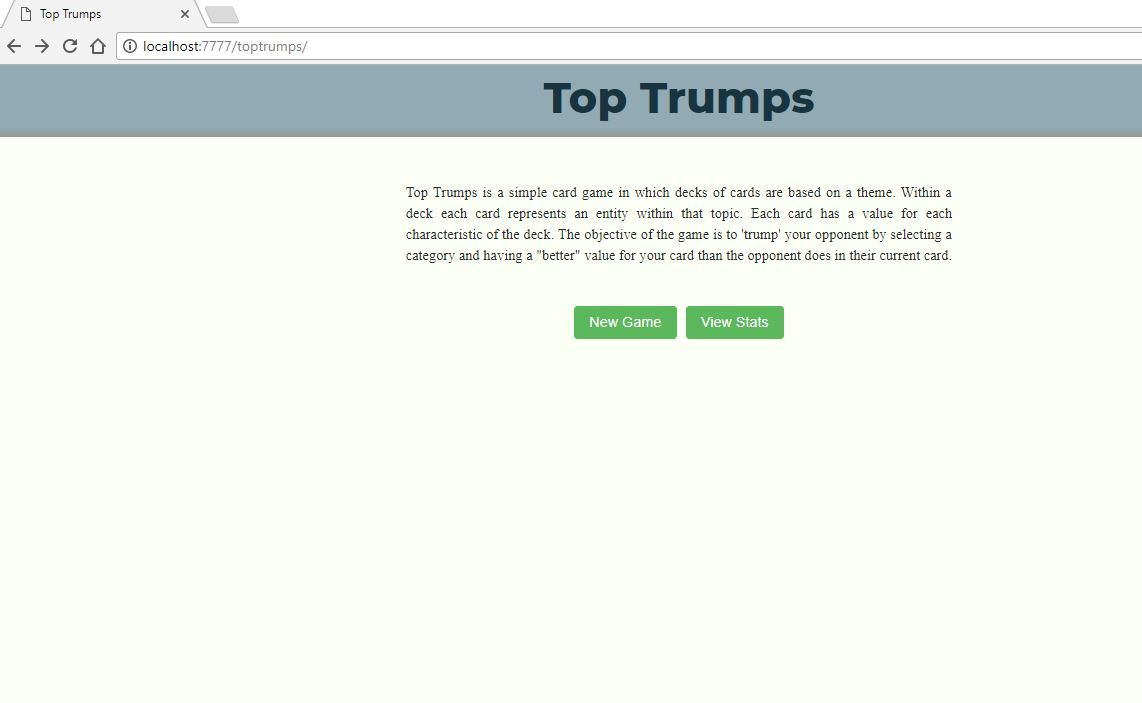
\includegraphics[width=0.8\textwidth]{S0200_MainMenu}
	\captionof{figure}{Main menu of the online mode.}
	\label{figure:online_menu}
\end{center}
\begin{center}
	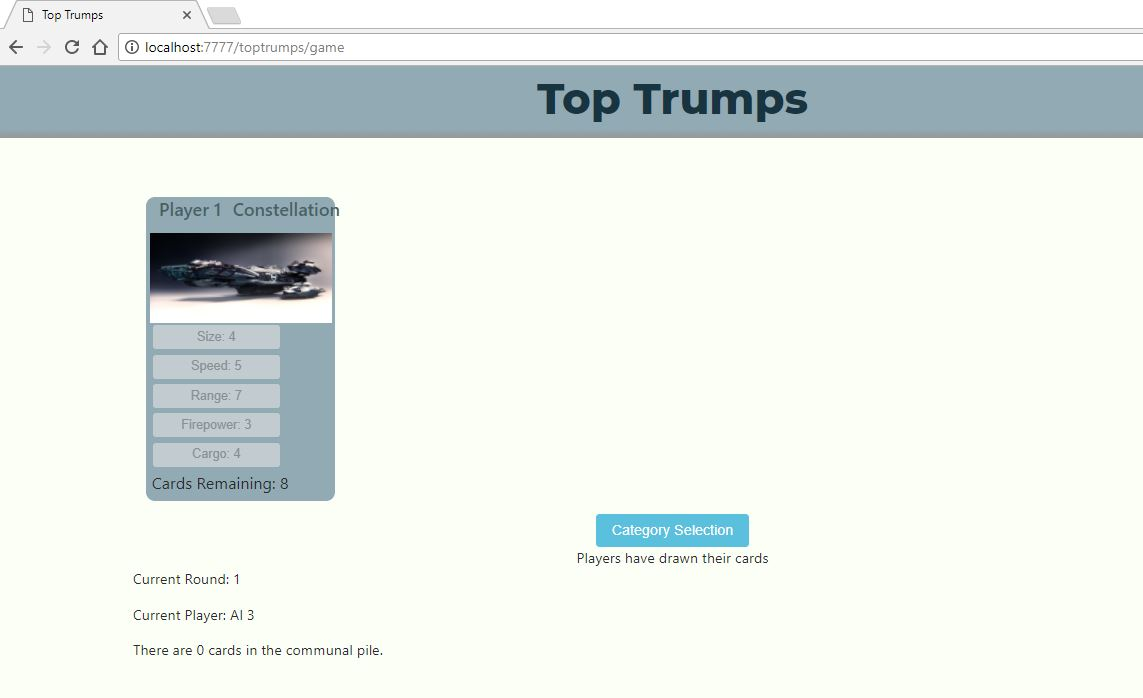
\includegraphics[width=0.8\textwidth]{S0220_RoundSet}
	\captionof{figure}{Initialised game, ready to start.}
	\label{figure:readyStart}
\end{center}
\begin{center}
	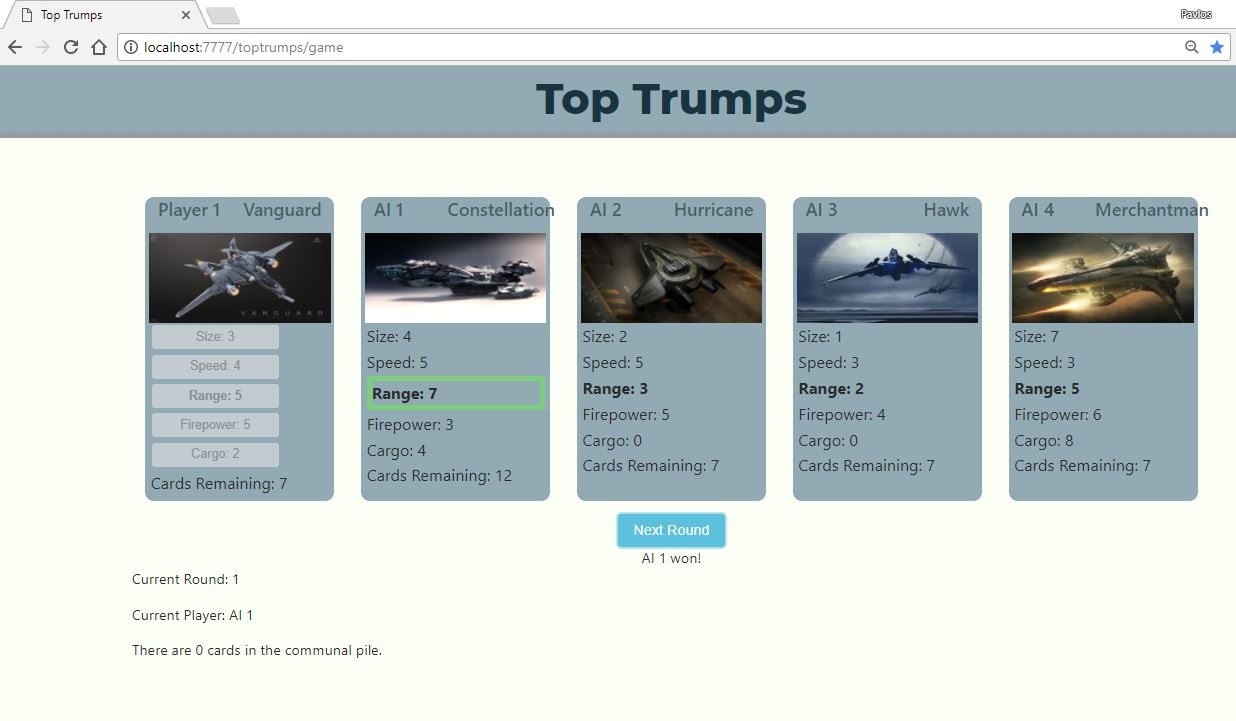
\includegraphics[width=0.8\textwidth]{S0220_RoundOutcome}
	\captionof{figure}{Round winner. With bold is the selected category and with the green rectangular indicates the winner}
	\label{figure:online_play}
\end{center}
\begin{center}
	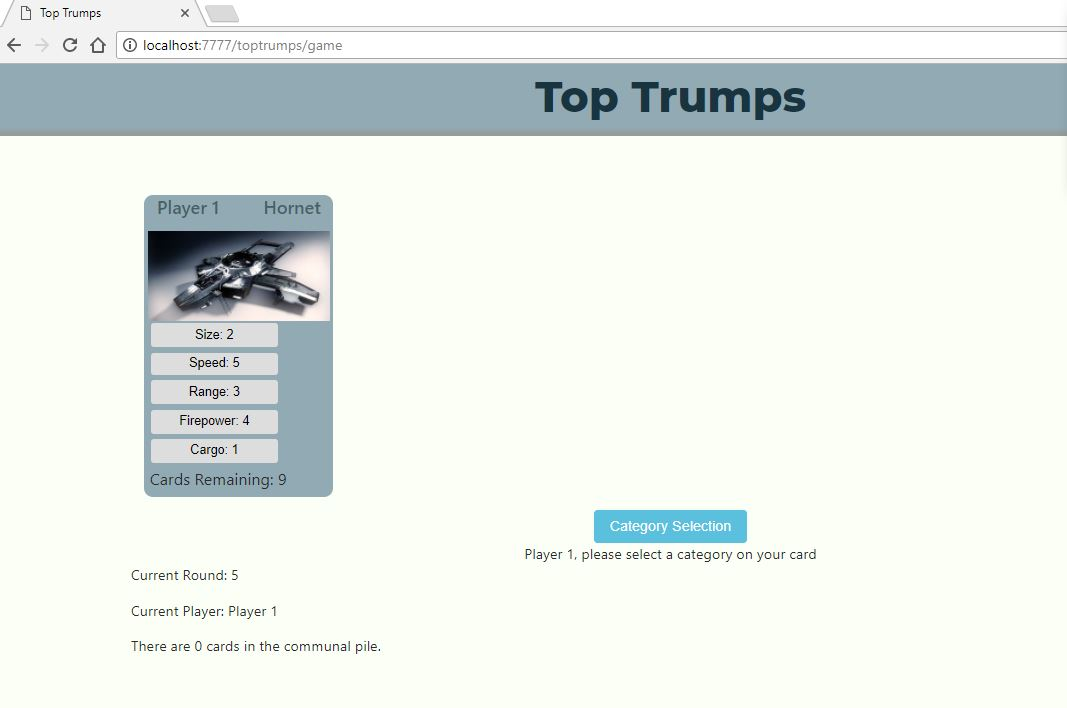
\includegraphics[width=0.8\textwidth]{S0220_selectCategory}
	\captionof{figure}{Round winner is the human player and must select a category before the game proceeds.}
	\label{figure:online_selectCategory}
\end{center}
\begin{center}
	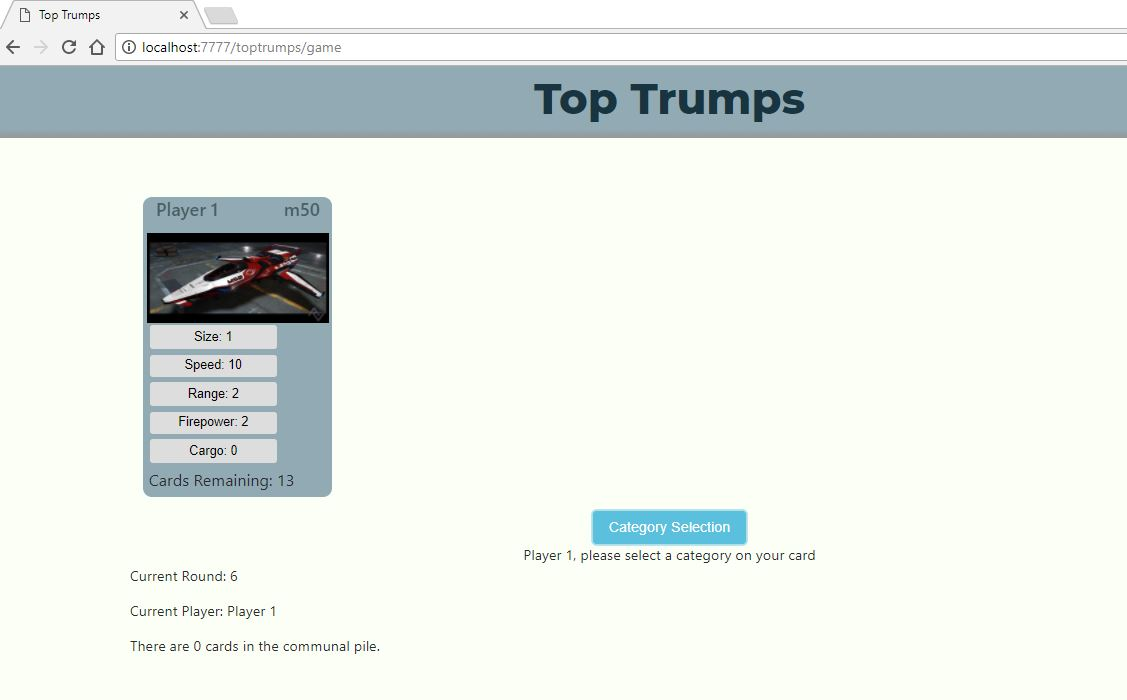
\includegraphics[width=0.8\textwidth]{S0230_HumanActive}
	\captionof{figure}{Below the main button displays the selected category and who was active player.}
	\label{figure:online_humanRound}
\end{center}
\begin{center}
	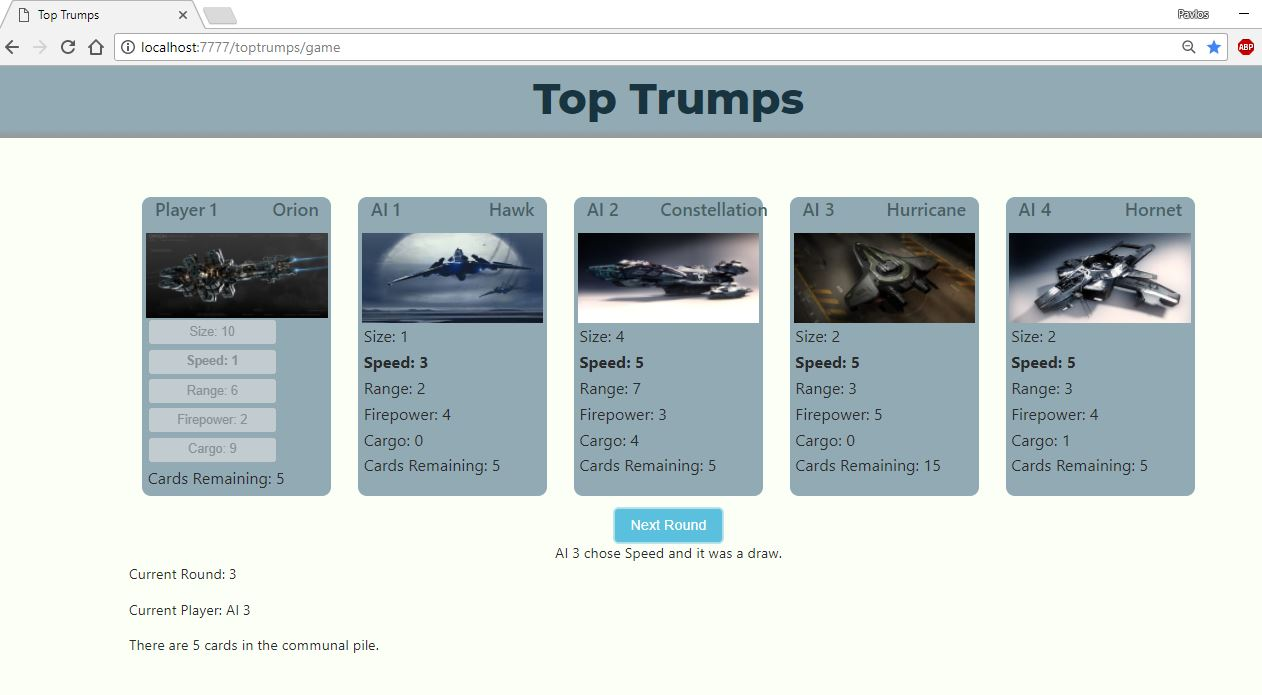
\includegraphics[width=0.8\textwidth]{S0240_DrawOnline}
	\captionof{figure}{Draw outcome. With bold is the selected category, there is no green indication of winner and the communal pile stores the cards of the players who are still in the game.}
	\label{figure:drawOnline}
\end{center}
\begin{center}
	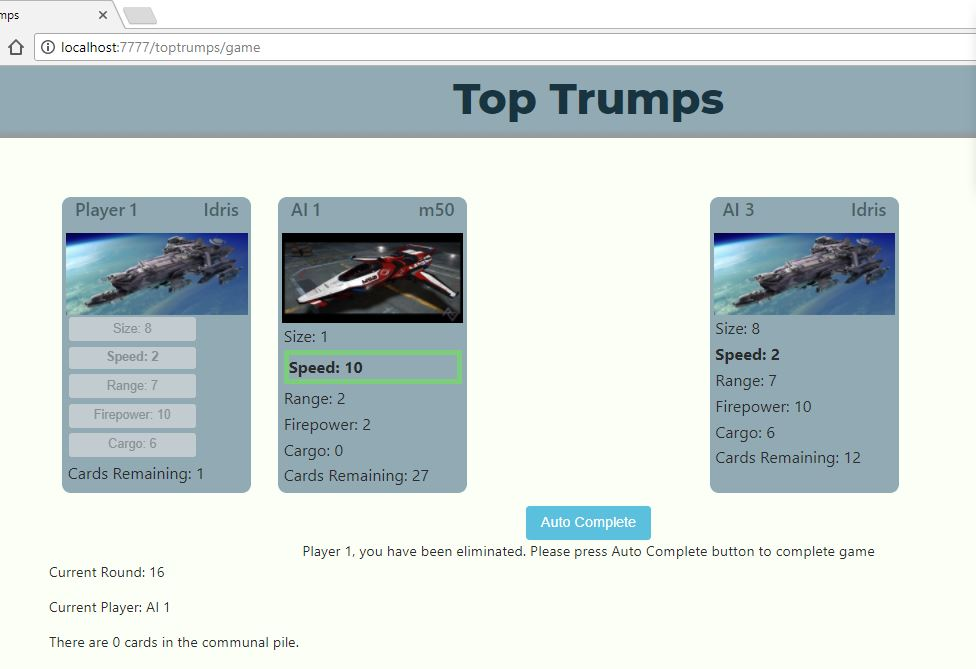
\includegraphics[width=0.8\textwidth]{S0250_AutoComplete}
	\captionof{figure}{If the human player is eliminated the auto-complete button appears.}
	\label{figure:autoComplete}
\end{center}
\begin{center}
	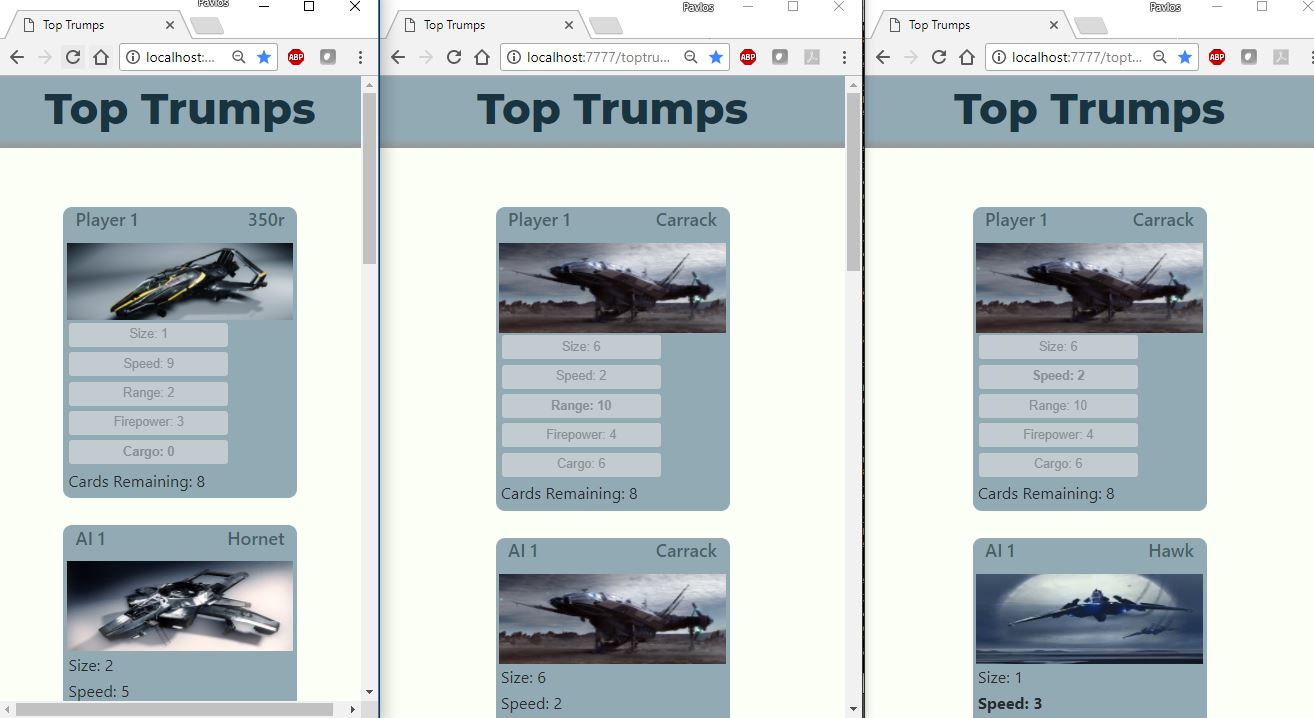
\includegraphics[width=0.8\textwidth]{S0250_MultipleGames}
	\captionof{figure}{Multiple games can exist simultaneously in different tabs with game index.}
	\label{figure:multipleGames}
\end{center}
\begin{center}
	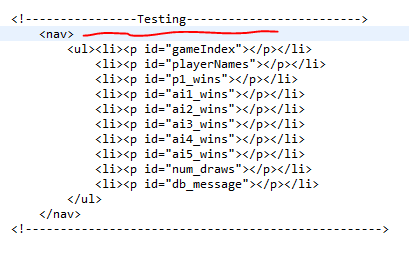
\includegraphics[width=0.8\textwidth]{onlineTesting}
	\captionof{figure}{The above variables were not hidden during the development of the, in order to test the functionality of the online mode.}
\end{center}
\begin{center}
	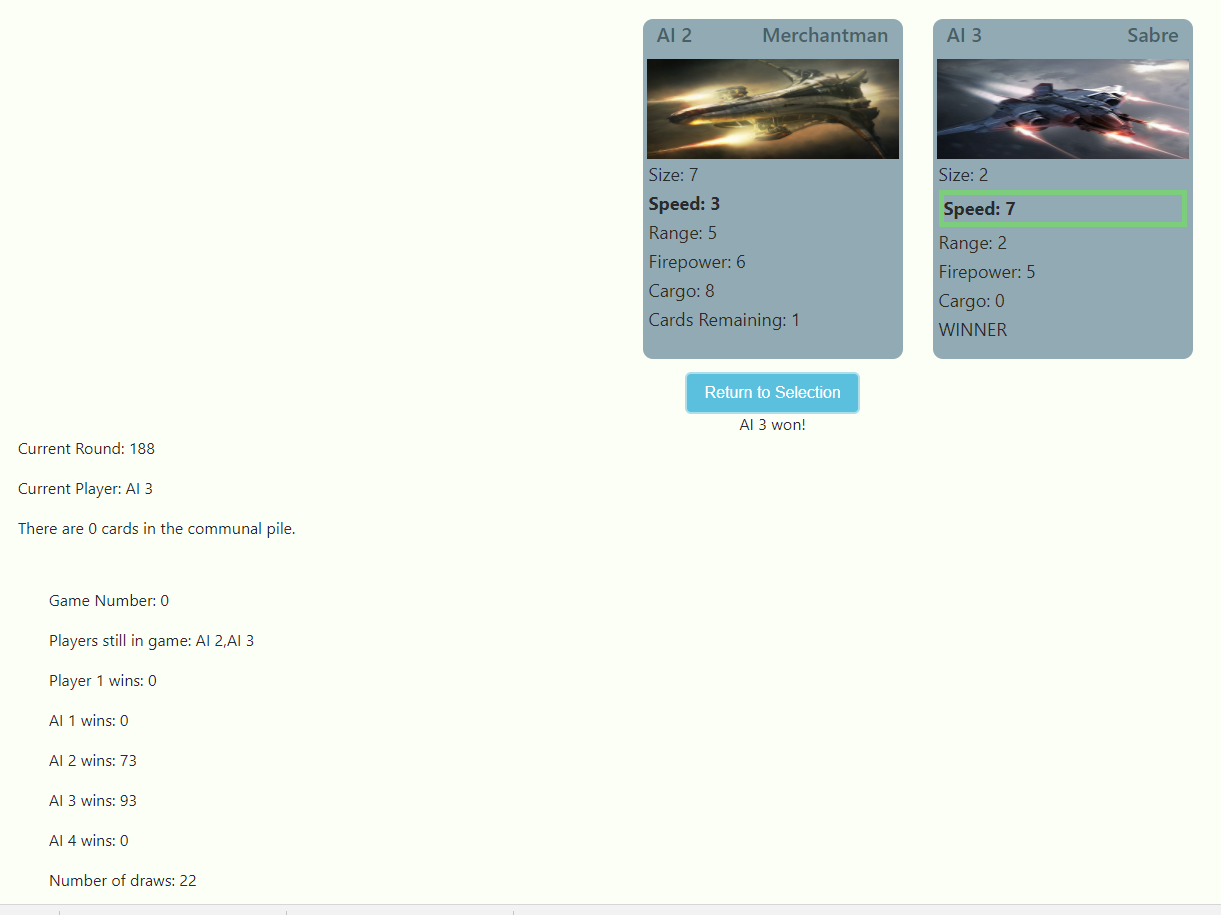
\includegraphics[width=0.8\textwidth]{onlineTesting_2}
	\captionof{figure}{This figure is connected with the figure above and provides a clear understanding about the testing.}
\end{center}
\begin{center}
    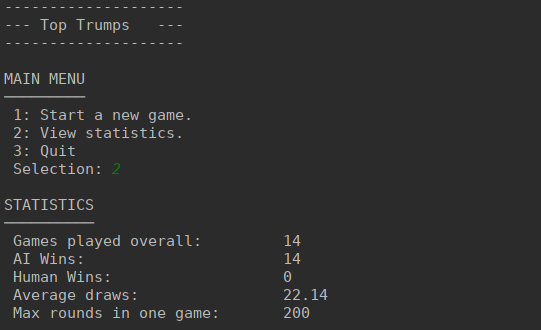
\includegraphics[width=0.8\textwidth]{cmd_stats}
    \captionof{figure}{Command Line Statistics View}
    \label{figure:cmd_stats}
\end{center}
\begin{center}
    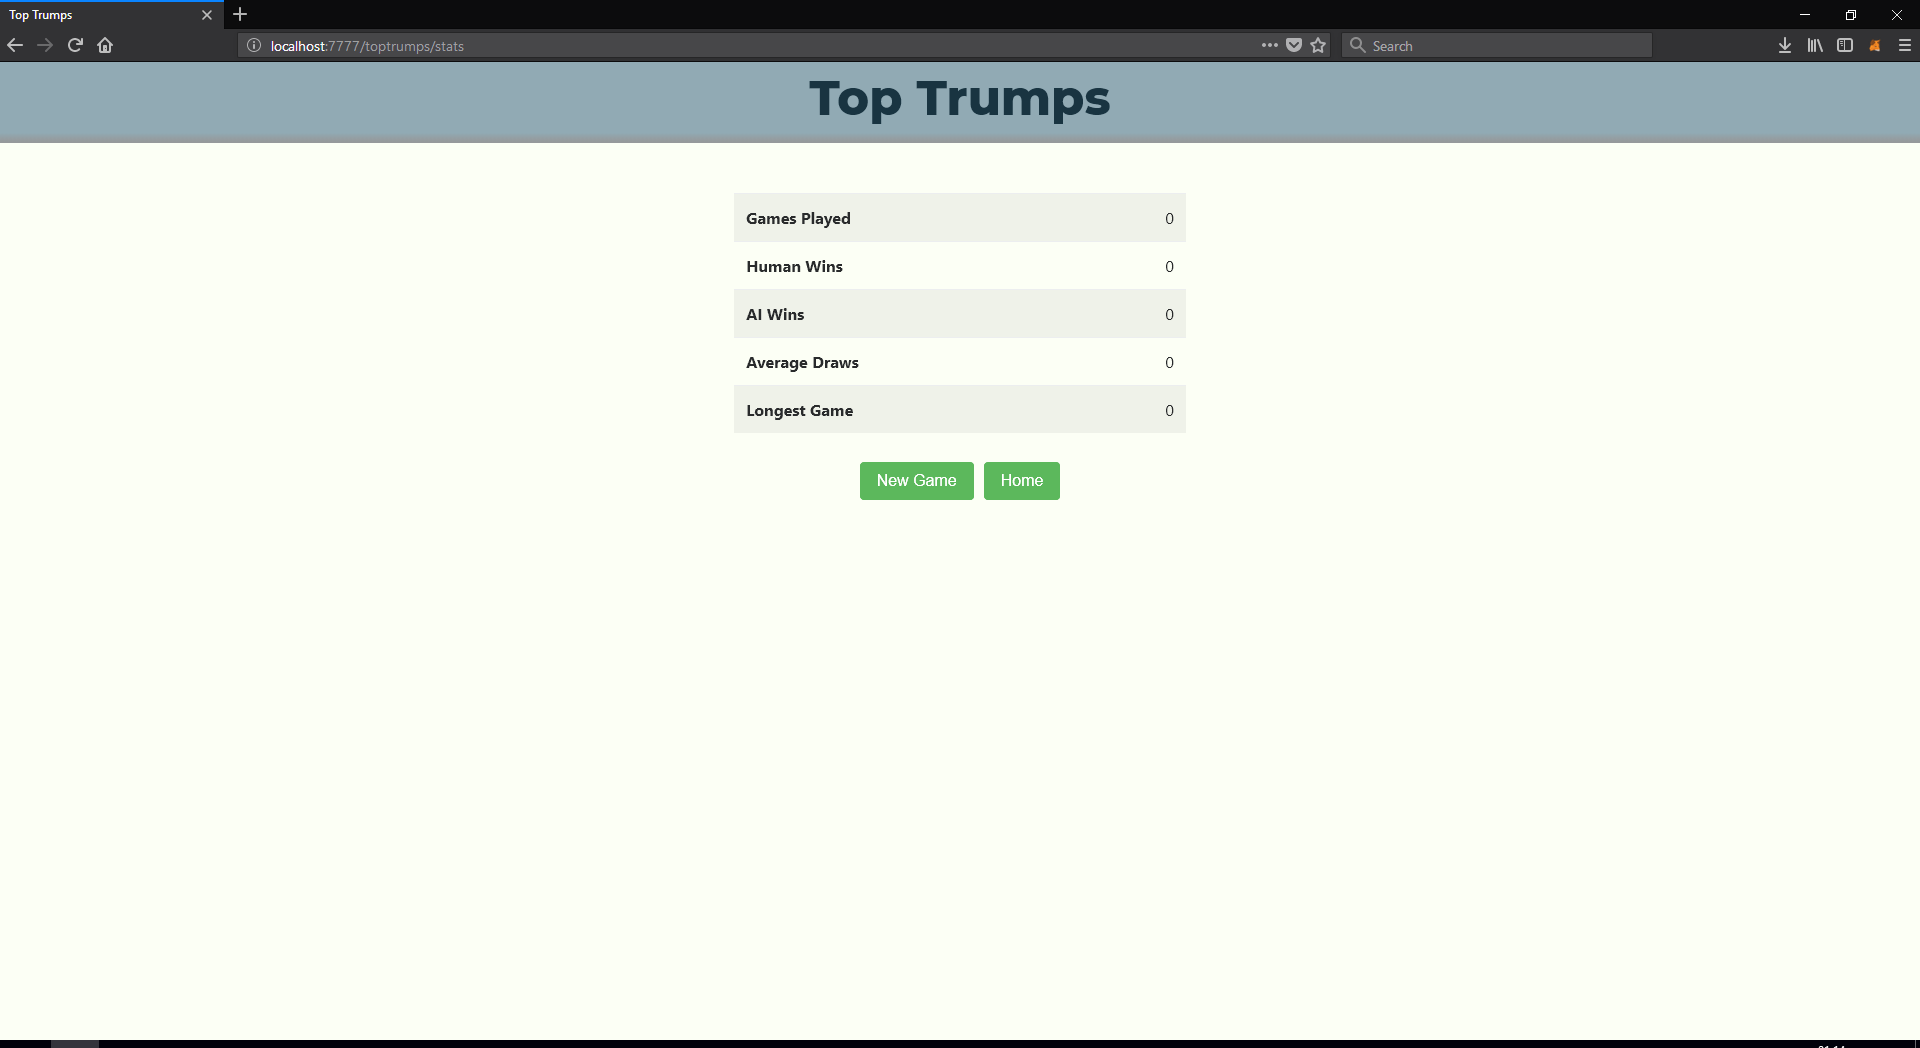
\includegraphics[width=0.8\textwidth]{online_stats}
    \captionof{figure}{Online Statistics View}
    \label{figure:online_stats}
\end{center}
\begin{center}
    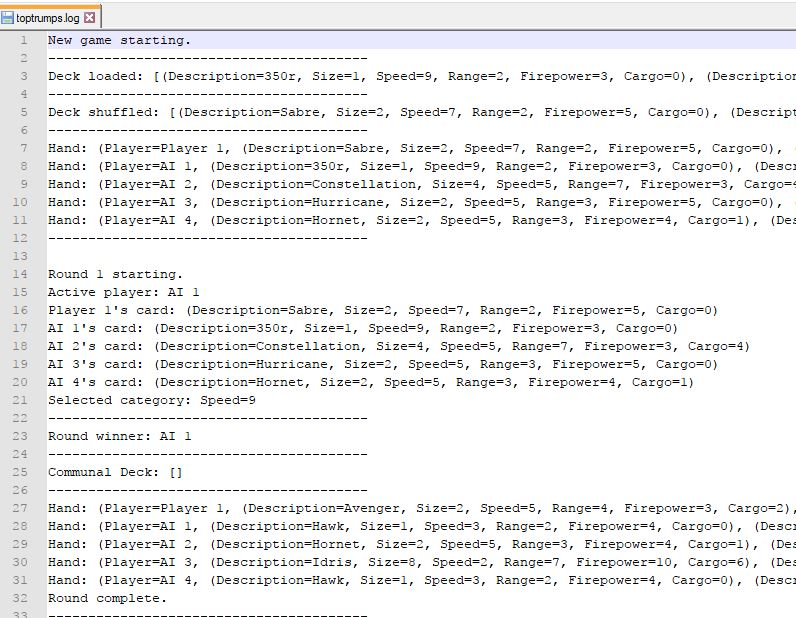
\includegraphics[width=0.8\textwidth]{S0020_testlog}
    \captionof{figure}{All the details of the game is inside the test log file.}
    \label{figure:testlog}
\end{center}
\begin{center}
    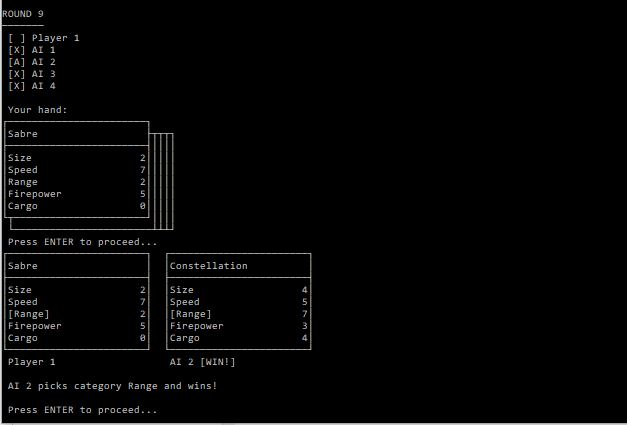
\includegraphics[width=0.8\textwidth]{S0050_showEliminated}
    \captionof{figure}{The program shows who is eliminated from the game with a X mark inside the brackets.}
    \label{figure:eliminated}
\end{center}


\end{appendices}

\end{document}